\documentclass[12pt,a4paper]{report}

\usepackage[utf8]{inputenc}
\usepackage[T1]{fontenc}
\usepackage[french]{babel}

\usepackage{newtxtext}
\usepackage{newtxmath}

\usepackage{lettrine}
\usepackage{float}
\usepackage{fancyhdr}
\usepackage{array}
\usepackage{setspace}
\onehalfspacing
\usepackage{graphicx}
\usepackage{xcolor}

\usepackage{hyperref}
\usepackage[all]{hypcap}
\usepackage{csquotes}

\usepackage[none]{hyphenat}
\usepackage{enumitem}

% style/style.tex (NO \documentclass or \begin{document} here!)
\usepackage{geometry}
\geometry{
  left=25mm,
  right=20mm,
  top=20mm,
  bottom=20mm,
  headheight=14pt
}

\usepackage{xcolor}
\definecolor{Primary}{RGB}{0,60,120}    
\definecolor{Secondary}{RGB}{0,120,150} 
\definecolor{Accent}{RGB}{255,200,0}    
\definecolor{Dark}{RGB}{30,30,30}

\newcommand{\Institut}{Institut Supérieur d’Informatique et du Multimédia de Sfax}
\newcommand{\Departement}{Département Informatique}
\newcommand{\Titre}{Application Web pour la Gestion des Immobilisations}
\newcommand{\TitreCourt}{Gestion des Immobilisations}
\newcommand{\Auteurs}{Mohamed Ali HAMDI}
\newcommand{\Encadrants}{Encadrant professionnel : M. Issam SOUSSI}
\newcommand{\Annee}{Année universitaire 2025/2026}

\usepackage{mdframed}
\usepackage{titlesec}

\titleformat{\chapter}[display]
  {\bfseries\Large\color{Primary}}
  {\filright\tiny\bfseries\MakeUppercase{\chaptername}~\thechapter}
  {1ex}
  {\titlerule[0.8pt]\vspace{1ex}\filright\scshape}
  [\vspace{1ex}\titlerule]

\newcommand{\HRule}{\noindent\color{Primary}\rule{\linewidth}{0.8pt}}

\hypersetup{colorlinks=true,linkcolor=Primary,urlcolor=Primary,citecolor=Primary}

\pagestyle{fancy}
\fancyhf{}
\fancyhead[L]{\small \nouppercase{\leftmark}}
\fancyhead[R]{}
\fancyfoot[C]{\thepage}

\usepackage[backend=biber,style=ieee]{biblatex}
\addbibresource{references.bib}

\makeatletter
\newcommand{\emptypage}[1]{%
  \cleardoublepage
  \begingroup
  \let\ps@plain\ps@empty
  \pagestyle{empty}
  #1
  \cleardoublepage
  \endgroup
}
\makeatother

\begin{document}

\pagenumbering{arabic}

\begin{titlepage}
  \begin{titlepage}
\begin{center}

\begin{minipage}[c]{0.48\linewidth}
   \flushleft
   
\includegraphics[height=2.0cm, keepaspectratio]{../../assets/logoISIMS.png}
\end{minipage}
\hfill
\begin{minipage}[c]{0.48\linewidth}
   \flushright
   
\includegraphics[height=2.0cm, keepaspectratio]{../../assets/logoSTEG.png}
\end{minipage}

\vspace{0.5cm}

{\small
RÉPUBLIQUE TUNISIENNE\\
MINISTÈRE DE L'ENSEIGNEMENT SUPÉRIEUR ET DE LA RECHERCHE SCIENTIFIQUE\\
Université de Sfax\\
\textbf{\large Institut Supérieur d'Informatique et du Multimédia de Sfax}\\
}

\vspace{0.6cm}
\hrule height 1pt
\vspace{0.6cm}

{\Large \textbf{\scshape RAPPORT DE PROJET DE FIN D'ANNÉE}}\\[0.6cm]

{\large Présenté à}\\[0.1cm]
{\textbf{L'Institut Supérieur d'Informatique et du Multimédia de Sfax}}\\[0.4cm]

{\large Effectué à}\\[0.1cm]
{\textbf{La Société Tunisienne de l'Électricité et du Gaz (STEG)}}\\[0.5cm]

\textbf{Spécialité :}\\
{\large \textbf{Licence en Big Data et Analyse de Données}}\\[0.8cm]

\hrule height 1pt
\vspace{0.4cm}
{\Large \textbf{Sujet :}} \\[0.3cm]
{\LARGE \textbf{Application Web pour la Gestion des Immobilisations}}
\vspace{0.4cm}
\hrule height 1pt

\vspace{0.6cm}
{\large Période du stage : du 08/06/2026 au 07/07/2026}\\[1cm]

\begin{minipage}[t]{0.45\linewidth}
   \flushleft
   \textbf{Réalisé par :}\\
   Mohamed Ali HAMDI
\end{minipage}
\hfill
\begin{minipage}[t]{0.45\linewidth}
   \flushright
   \textbf{Sous la direction de :}\\
   M. Issam SOUSSI
\end{minipage}

\vfill

{\large Année universitaire : 2025/2026}

\end{center}
\end{titlepage}
\end{titlepage}

\clearpage
\thispagestyle{empty}
\chapter*{Remerciements}
\addcontentsline{toc}{chapter}{Remerciements}

C'est avec une profonde gratitude et un grand respect que j'adresse mes remerciements à toutes les personnes qui ont contribué au bon déroulement de ce projet de fin d'année.

\clearpage
\tableofcontents

\clearpage
\listoffigures

\clearpage
\chapter*{Introduction Générale}
\addcontentsline{toc}{chapter}{Introduction Générale}

À l'ère de la transformation numérique, la modernisation des outils de gestion constitue un levier de performance incontournable pour les grandes structures industrielles. Les systèmes d'information traditionnels, souvent basés sur des processus manuels ou des outils décentralisés, montrent aujourd'hui leurs limites face aux exigences de réactivité, de traçabilité et de sécurité des organisations modernes. La gestion des actifs physiques et du patrimoine matériel représente, à ce titre, un enjeu stratégique majeur pour optimiser l'exploitation des ressources et garantir un suivi rigoureux des investissements.

C'est dans ce contexte que s'inscrit le présent projet, réalisé au sein de la Société Tunisienne de l'Électricité et du Gaz (STEG). En tant qu'acteur national pivot du secteur énergétique, la société s'appuie sur une infrastructure technique et immobilière d'envergure, répartie sur de nombreuses directions régionales et locaux de stockage. L'absence d'une solution logicielle unifiée et accessible en temps réel pour le suivi des immobilisations, telles que les parcs de véhicules, les équipements électriques ou les structures physiques, engendre des difficultés d'inventaire et complexifie la coordination entre les différents services responsables.

L'objectif principal de ce travail consiste donc à concevoir et à développer une application web dédiée à la gestion automatisée des immobilisations. Cette solution doit permettre de recenser de manière centralisée le patrimoine de la structure, de suivre avec précision l'état et la localisation de chaque type de matériel, et de fluidifier le processus de contrôle des inventaires. Pour répondre aux besoins de sécurité et de répartition des tâches au sein de l'entreprise, la plateforme doit également proposer un contrôle d'accès strict basé sur différents profils d'utilisateurs.

Pour rendre compte de la réalisation de ce système, le présent rapport s'organise en plusieurs chapitres complémentaires. La première partie expose le contexte général du projet et présente la structure d'accueil ainsi que la problématique identifiée. La deuxième partie est consacrée à l'analyse détaillée des exigences fonctionnelles et non fonctionnelles, tout en spécifiant les profils des acteurs et l'écosystème logiciel retenu. Enfin, les dernières sections détaillent la phase de conception technique à travers la modélisation des bases de données et des processus, avant de présenter l'implémentation logicielle, les interfaces de l'application et les résultats des tests d'intégration.

\clearpage
\chapter{Contexte Général}

\section{Introduction}

Ce chapitre pose le cadre institutionnel du projet en présentant la structure d’accueil au sein de laquelle le travail a été effectué. L'étude débute par un historique et une vue d'ensemble des missions stratégiques de l'entreprise nationale en charge de l'énergie, avant de détailler l'organisation technique de la direction régionale de rattachement. Cette immersion permet de mieux appréhender les flux opérationnels existants et de situer l'application développée dans son environnement organisationnel réel.

\section{STEG}

\subsection{Présentation de la société}

À la veille de l'indépendance de la Tunisie, l'activité électrique nationale était fragmentée et gérée par sept sociétés concessionnaires distinctes. Ces structures assuraient l'alimentation des principales régions du pays avec une puissance totale installée de près de 100 MW pour une production annuelle d'environ 240 GWh. 

Dans le but d'harmoniser, de centraliser et d'optimiser le secteur de l'énergie stratégique, l'État tunisien a promulgué la loi numéro 62-8 du 3 avril 1962, portant création de la Société Tunisienne de l'Électricité et du Gaz. Cette institution s'est vu confier le monopole de la production, du transport et de la distribution de l'électricité ainsi que du gaz sur l'ensemble du territoire national.

Les missions fondamentales assignées à l'entreprise s'articulent autour de l'électrification globale du pays, de l'extension progressive du réseau de gaz naturel et de la réalisation d'infrastructures d'envergure. À ce titre, la structure assure la responsabilité technique et commerciale de l'approvisionement énergétique du marché national afin de répondre aux exigences croissantes des différents secteurs de consommation, qu'ils soient résidentiels, industriels ou tertiaires.

Sur le plan opérationnel, les activités couvrent la production de l'énergie électrique à partir de sources diversifiées telles que le thermique, l'hydraulique ou l'éolien, ainsi que la fabrication du Gaz de Pétrole Liquéfié. Le transit de cette énergie s'effectue via un réseau de transport composé de lignes et de postes à haute tension, relayé par un réseau de distribution à moyenne et basse tension assurant l'acheminement final auprès des usagers.

\subsection{Organigramme de la société}

\begin{figure}[H]
  \centering
  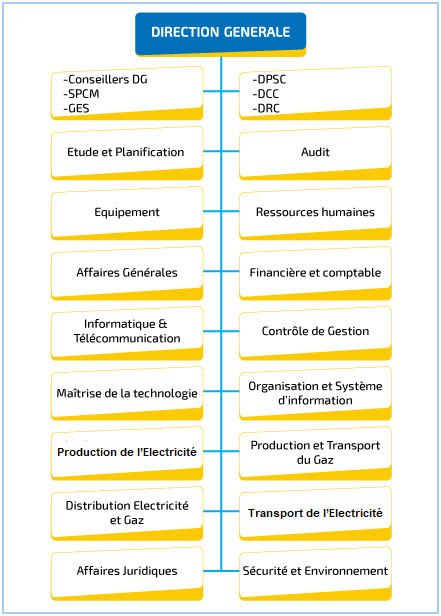
\includegraphics[width=0.9\textwidth]{../../assets/organigrammeSTEG.png}
  \caption{Organigramme général de la STEG} 
  \label{fig:organigrammeSTEG}
\end{figure}

\subsection{Département d'Exploitation Informatique Sud}

Le Département d'Exploitation Informatique Sud constitue l'entité technique pivot chargée de garantir la continuité, la sécurité et la performance des infrastructures informatiques pour les structures régionales. Ce service assure la supervision des systèmes de communication, l'administration des bases de données locales, ainsi que la maintenance du parc matériel et logiciel utilisé par les agents. C'est au sein de cet environnement technologique que s'est déroulée la conception de la solution, permettant d'aligner le développement de l'application sur les standards d'exploitation et les exigences de sécurité de la direction.

\subsection{Organigramme de la Département d'Exploitation Informatique Sud}

\begin{figure}[H]
  \centering
  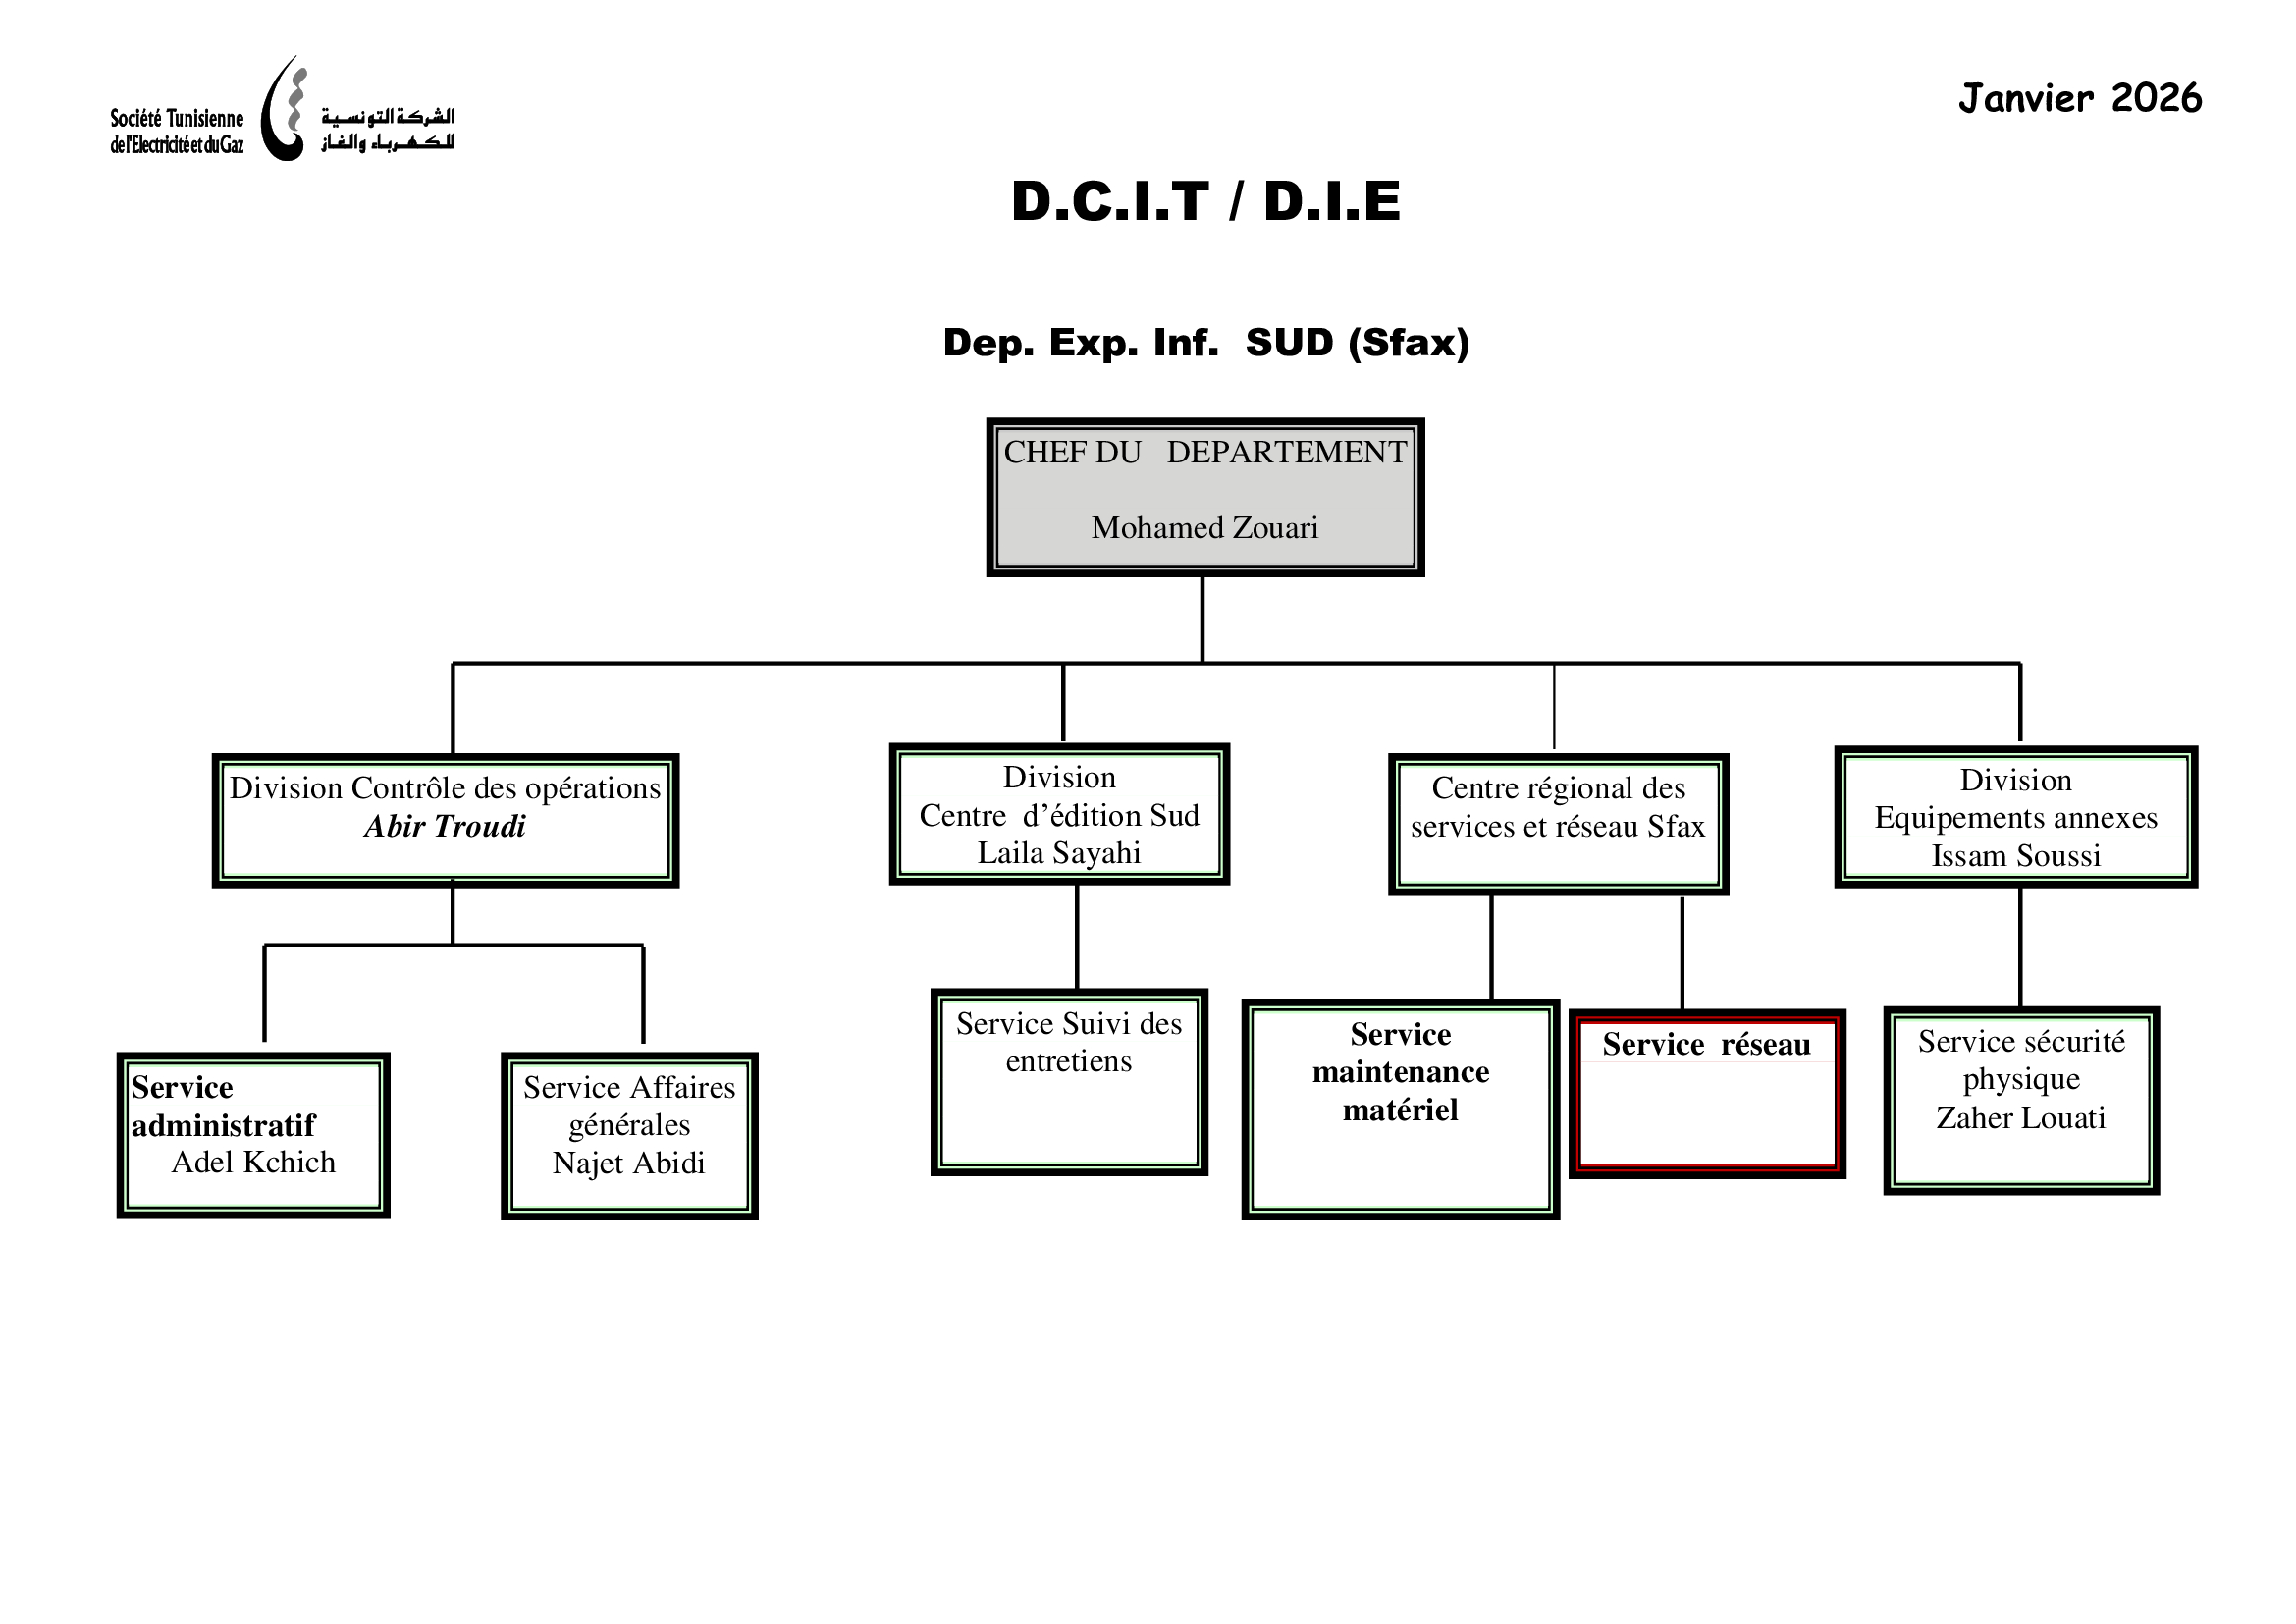
\includegraphics[width=0.9\textwidth]{../../assets/Organigramme-Dep-Exp-Sud.jpg}
  \caption{Organigramme général de la Département d'Exploitation Informatique Sud} 
  \label{fig:Organigramme-Dep-Exp-Sud}
\end{figure}

\clearpage
\chapter{Analyse des Exigences}

\section{Introduction}

Ce chapitre est dédié à l'analyse approfondie des besoins et des spécifications techniques indispensables à la conception du système de gestion. Cette phase préliminaire permet de cerner précisément le périmètre d'application du projet en identifiant l'ensemble des acteurs appelés à interagir avec la plateforme. La formalisation des exigences se structure autour de deux axes complémentaires : d'une part, la description des fonctionnalités opérationnelles attendues par la structure, et d'autre part, la définition des critères de qualité, de sécurité et de performance indispensables à la viabilité de la solution. Enfin, une présentation détaillée de l'écosystème technologique retenu vient compléter cette étude afin de poser les fondations techniques du développement futur.

\section{Identification des Acteurs}

Le système distingue plusieurs profils d'utilisateurs, chacun disposant de droits d'accès spécifiques adaptés à la gestion et au suivi du patrimoine de la société :

\begin{itemize}[label=$\bullet$]
   \item \textbf{Administrateur :} Prise en charge de la gestion globale du système, de la configuration des paramètres généraux et du contrôle des accès utilisateurs.
   \item \textbf{Chef du Centre Informatique :} Supervision d'ensemble des actifs technologiques, validation des inventaires et génération des rapports de synthèse.
   \item \textbf{Responsable de Services :} Suivi des affectations, coordination des inventaires périodiques et validation des mouvements internes au niveau des différents services.
   \item \textbf{Responsable Équipements :} Gestion du cycle de vie du matériel technique, de son enregistrement initial jusqu'à sa mise au rebut.
   \item \textbf{Gestionnaire de Voitures :} Suivi spécifique du parc roulant, incluant l'état de la flotte automobile, les affectations et la maintenance des véhicules.
   \item \textbf{Agent de Local :} Gestion et suivi des immobilisations affectées aux espaces physiques, bureaux et structures de la direction.
\end{itemize}

\section{Exigences Fonctionnelles}

Le système s'articule autour de plusieurs modules fonctionnels interconnectés permettant d'assurer la traçabilité complète et la gestion du cycle de vie du patrimoine de la structure.

Le premier module concerne la gestion des accès et de la sécurité. Le système doit garantir une authentification sécurisée pour chaque profil utilisateur. L'attribution des droits d'accès s'effectue de manière stricte, limitant la visibilité et les actions possibles sur l'application en fonction du rôle attribué à chaque agent lors de la configuration de son compte.

Le cœur de l'application repose sur le module de gestion du patrimoine physique et des locaux. Ce composant assure le recensement, la classification et le suivi rigoureux des structures, des directions, des rez-de-chaussée ainsi que de chaque localité physique. Chaque espace est répertorié avec ses caractéristiques structurelles afin de servir de point d'ancrage aux immobilisations.

Le module de gestion du matériel électrique et technique permet l'enregistrement complet de chaque équipement. Le système prend en charge le suivi de l'état opérationnel, la localisation exacte dans les différents bâtiments et l'affectation aux différents services. Il conserve l'historique complet des mouvements et des changements d'état pour chaque immobilisation technique.

Le volet relatif au parc roulant est pris en charge par le module de gestion des véhicules. Ce bloc fonctionnel assure le suivi de la flotte automobile de la société, l'enregistrement des spécificités techniques de chaque véhicule, ainsi que le contrôle des affectations par direction et par utilisateur responsable.

Enfin, un module dédié à l'inventaire et aux bilans offre des fonctionnalités de synthèse. Le système permet l'édition d'états d'inventaire périodiques par local ou par nature de matériel, facilitant ainsi les opérations de contrôle physique, la détection des anomalies de placement et la prise de décision concernant la mise au rebut ou le renouvellement des actifs.

\section{Exigences Non Fonctionnelles}

Les exigences non fonctionnelles définissent les critères de qualité, de performance et de contraintes techniques indispensables pour garantir la viabilité et l'efficacité opérationnelle du système.

La sécurité constitue un pilier fondamental de l'application. Le système doit assurer une protection rigoureuse des données relatives au patrimoine de la société à travers un chiffrement des mots de passe et des communications. Le contrôle des sessions doit empêcher toute interception ou accès non autorisé, garantissant que chaque utilisateur évolue exclusivement dans la limite des droits liés à son profil.

La performance et la disponibilité de la plateforme sont essentielles pour soutenir le travail quotidien des équipes. L'application doit afficher des temps de réponse optimaux lors de l'exécution des requêtes de recherche ou de la génération des états d'inventaire, même en période de forte sollicitation. Une architecture stable doit maximiser le taux de disponibilité afin de permettre un accès continu aux informations du parc d'immobilisations.

\section{Environnement de Travail Logiciel}

Les technologies et outils logiciels suivants ont été employés pour la réalisation de ce projet :

\begin{itemize}[label=$\bullet$]
   \item \textbf{Langages Web (Front-end) :}
   \begin{itemize}[label=$\circ$]
     \item \textbf{HTML5 :} Permet de structurer le contenu et de définir l'architecture des pages web.
     \item \textbf{CSS3 :} Assure la mise en forme, le design et le rendu visuel de l'interface utilisateur.
     \item \textbf{JavaScript :} Apporte de la dynamisation et de l'interactivité aux éléments des pages web.
   \end{itemize}
   
   \item \textbf{Langage côté serveur (Back-end) :}
   \begin{itemize}[label=$\circ$]
     \item \textbf{PHP :} Gère la logique applicative, le traitement des requêtes et la communication avec le serveur.
   \end{itemize}
   
   \item \textbf{Gestion de données :}
   \begin{itemize}[label=$\circ$]
     \item \textbf{MySQL :} Système de gestion de base de données relationnelle utilisé pour stocker et organiser les informations de manière sécurisée.
     \item \textbf{phpMyAdmin :} Interface graphique Web qui simplifie l'administration et la manipulation des bases de données MySQL.
   \end{itemize}
   
   \item \textbf{Serveur local :}
   \begin{itemize}[label=$\circ$]
     \item \textbf{XAMPP :} Environnement de développement local complet et multiplateforme, incluant Apache, MariaDB et PHP, assurant la gestion des services nécessaires au fonctionnement du serveur web.
   \end{itemize}
   
   \item \textbf{Éditeur de code :}
   \begin{itemize}[label=$\circ$]
     \item \textbf{Visual Studio Code :} Environnement de développement léger et extensible, utilisé pour l'écriture et le débogage du code source.
   \end{itemize}
   
   \item \textbf{Conception des diagrammes :}
   \begin{itemize}[label=$\circ$]
     \item \textbf{PlantUML :} Serveur en ligne permettant de modéliser et de générer les diagrammes UML de manière programmable et structurée.
   \end{itemize}
\end{itemize}

\clearpage
\chapter{Conception}

\section{Introduction}

Ce chapitre présente la phase de conception technique de l'application. Cette étape cruciale permet de traduire les besoins fonctionnels identifiés précédemment en une architecture logicielle cohérente. À travers une modélisation utilisant le langage UML (Unified Modeling Language), nous détaillerons les interactions entre les différents acteurs et le système via les cas d'utilisation, la structure statique des données à travers le diagramme de classes, ainsi que la dynamique des processus métiers au moyen des diagrammes de séquences.

\clearpage
\section{Diagramme de Cas d'Utilisation Général}

\begin{figure}[H]
  \centering
  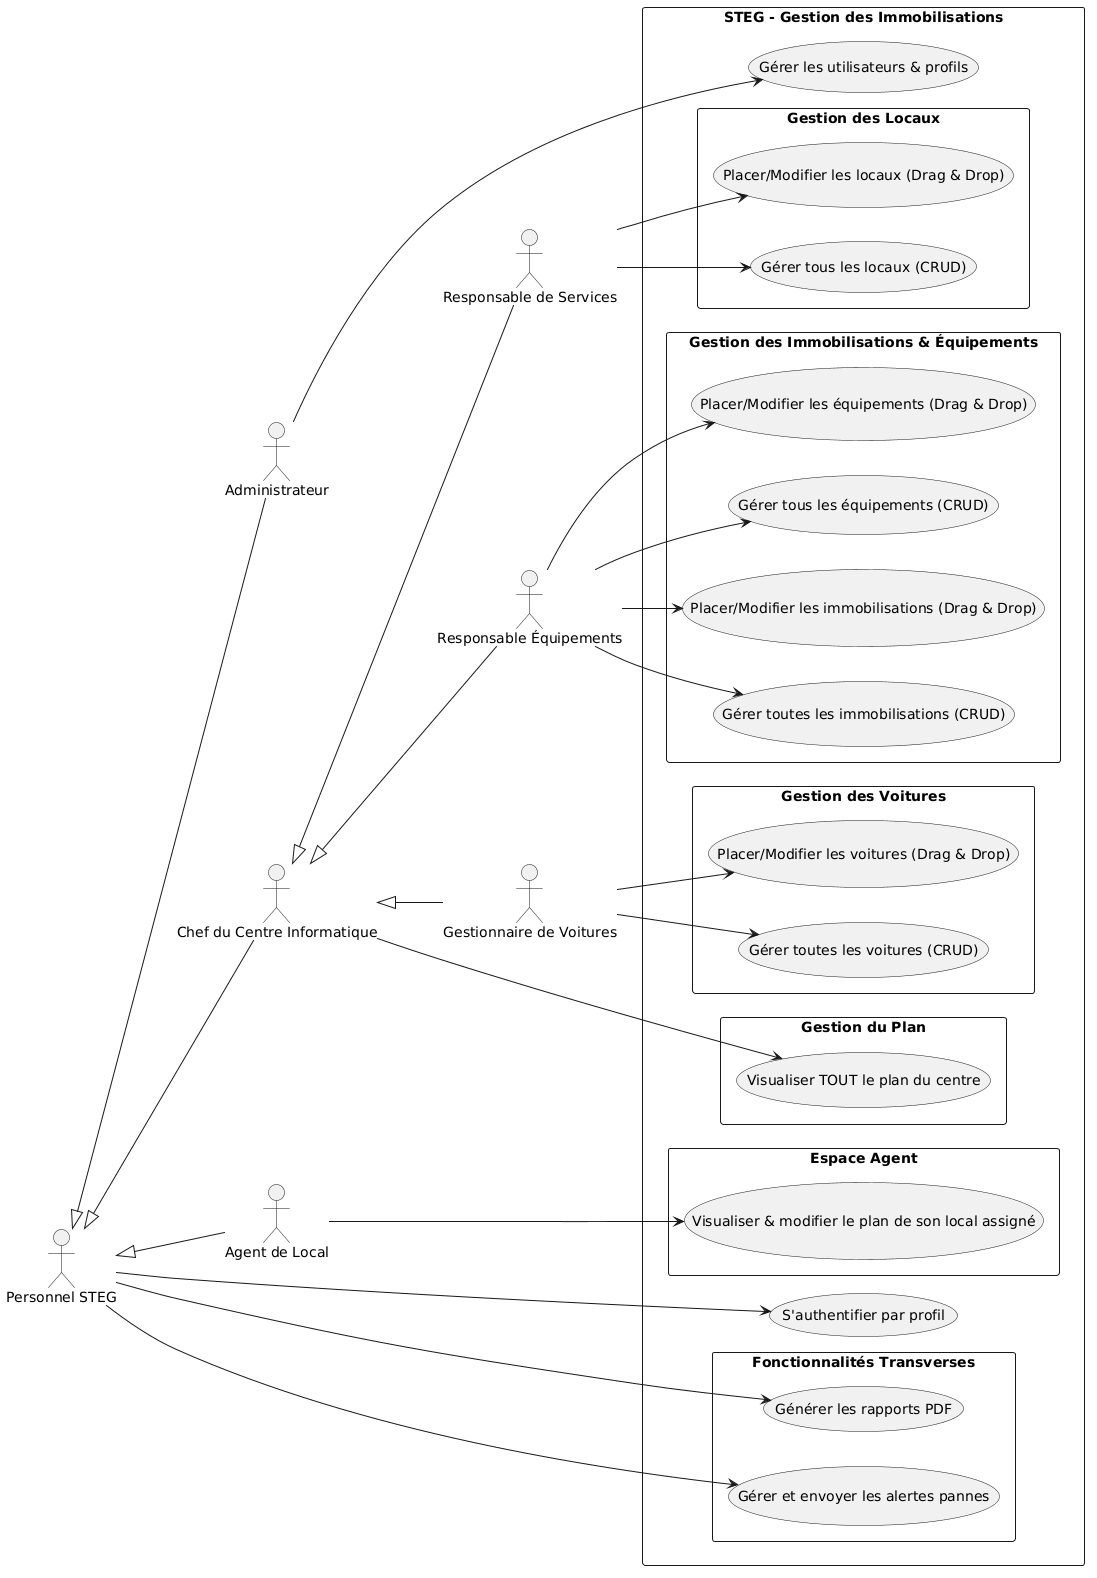
\includegraphics[width=\textwidth,height=0.75\textheight,keepaspectratio]{../../assets/use_case_diagram.png}
  \caption{Diagramme de cas d'utilisation général}
  \label{fig:use_case}
\end{figure}

\clearpage
\section{Diagramme de Classes Général}

\begin{figure}[H]
  \centering
  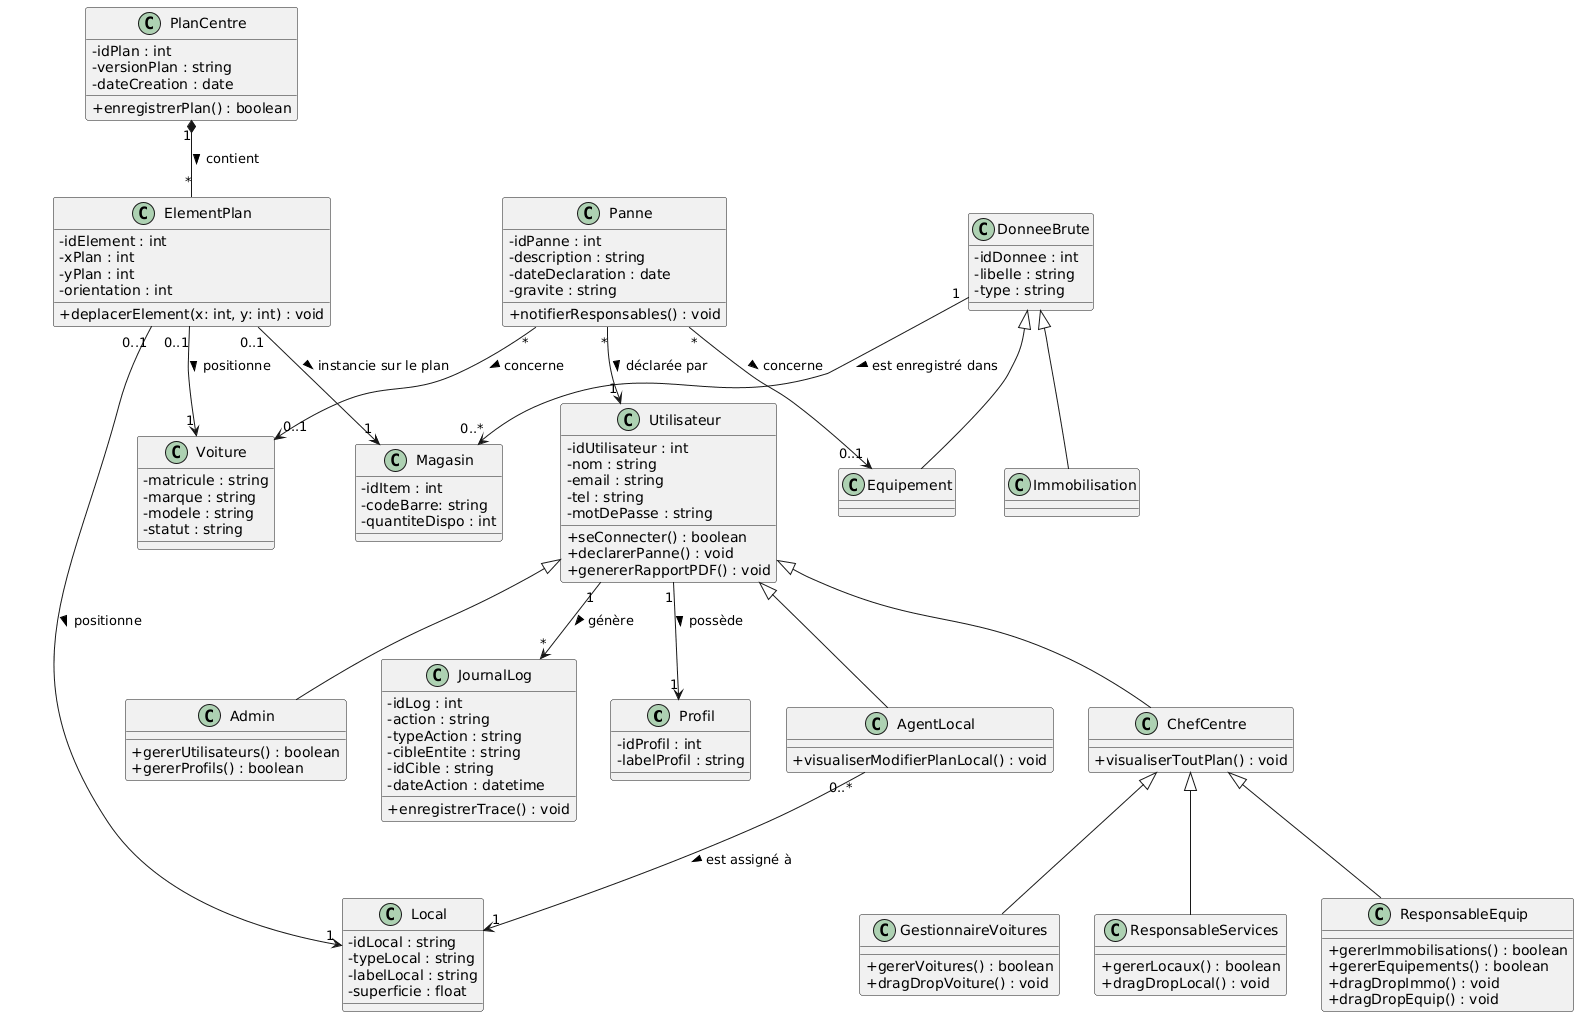
\includegraphics[width=\textwidth,height=0.75\textheight,keepaspectratio]{../../assets/class_diagram.png}
  \caption{Diagramme de classes général}
  \label{fig:class_diagram}
\end{figure}

\clearpage
\section{Diagramme de Séquences}

\subsection{Scénario d'Authentification (UC\_Auth)}

Le processus d'authentification représente le point d'entrée sécurisé de l'application. La cinématique ci-dessous détaille la vérification des identifiants ainsi que l'affectation dynamique de l'espace de travail en fonction du profil récupéré depuis la base de données.

\begin{figure}[H]
  \centering
  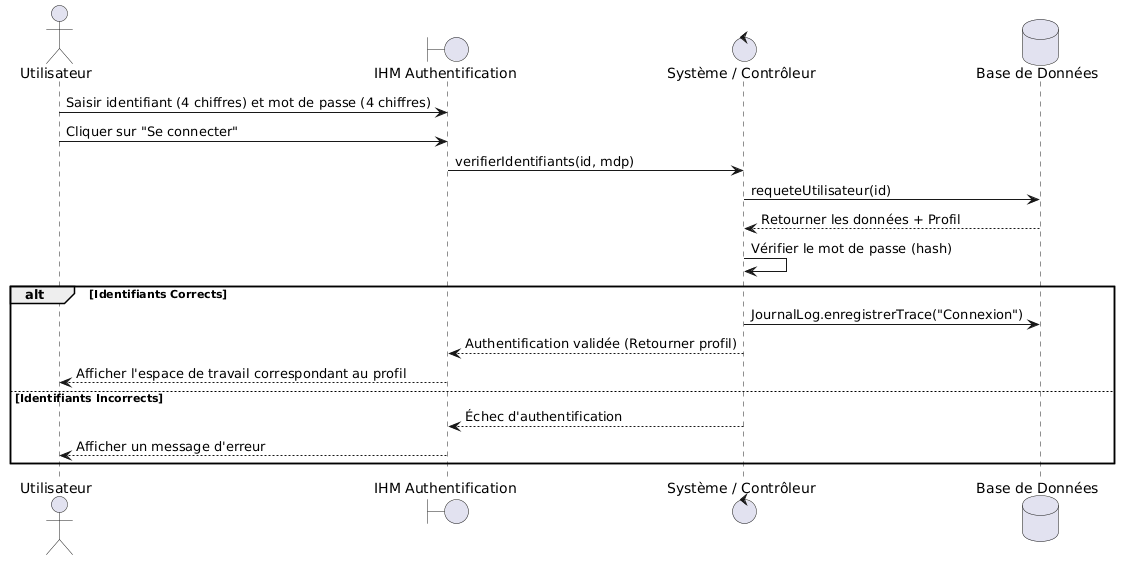
\includegraphics[width=\textwidth,height=0.65\textheight,keepaspectratio]{../../assets/seq_auth.png}
  \caption{Diagramme de séquence - Authentification par profil}
  \label{fig:seq_auth}
\end{figure}

\clearpage
\subsection{Scénario de Gestion des Utilisateurs (UC\_Admin\_System)}

Réservé exclusivement au profil Administrateur, ce cas d'utilisation décrit la logique de persistance lors de la création d'un nouveau compte utilisateur, incluant la vérification d'unicité de l'identifiant et l'écriture systématique dans le journal de traçabilité.

\begin{figure}[H]
  \centering
  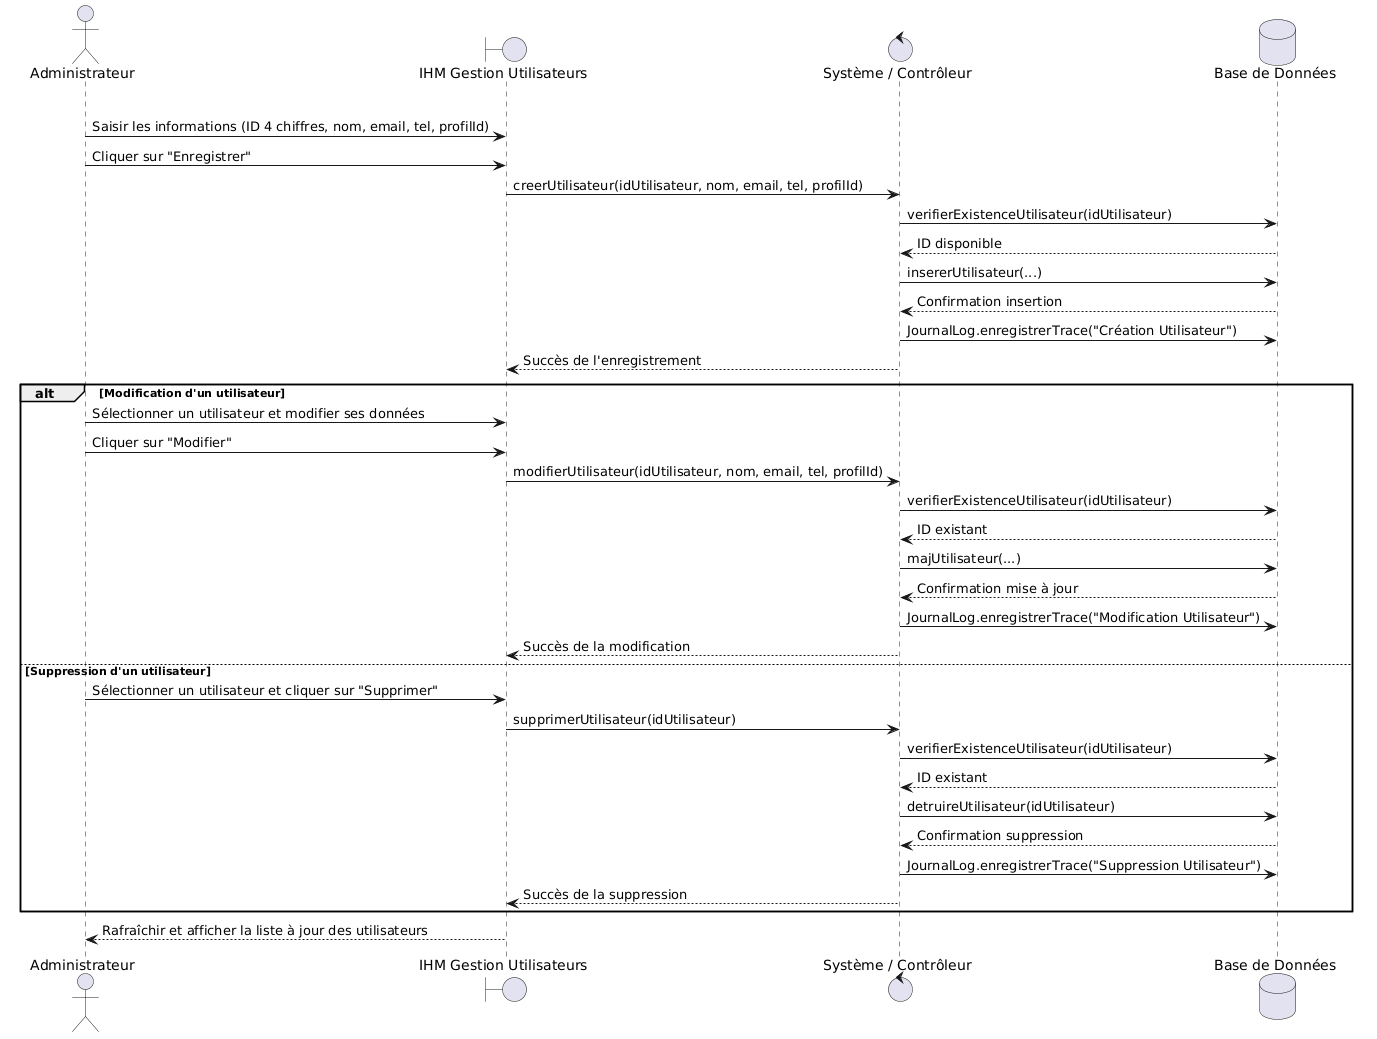
\includegraphics[width=\textwidth,height=0.65\textheight,keepaspectratio]{../../assets/seq_admin.png}
  \caption{Diagramme de séquence - Gestion des utilisateurs et profils}
  \label{fig:seq_admin}
\end{figure}

\clearpage
\subsection{Scénario de Visualisation du Plan}

Cette cinématique met en évidence le filtrage des données selon les privilèges de l'acteur connecté. Là où le Chef du Centre obtient une vue globale de l'infrastructure, l'Agent de Local ne reçoit que les éléments géographiques restreints à sa zone d'affectation.

\begin{figure}[H]
  \centering
  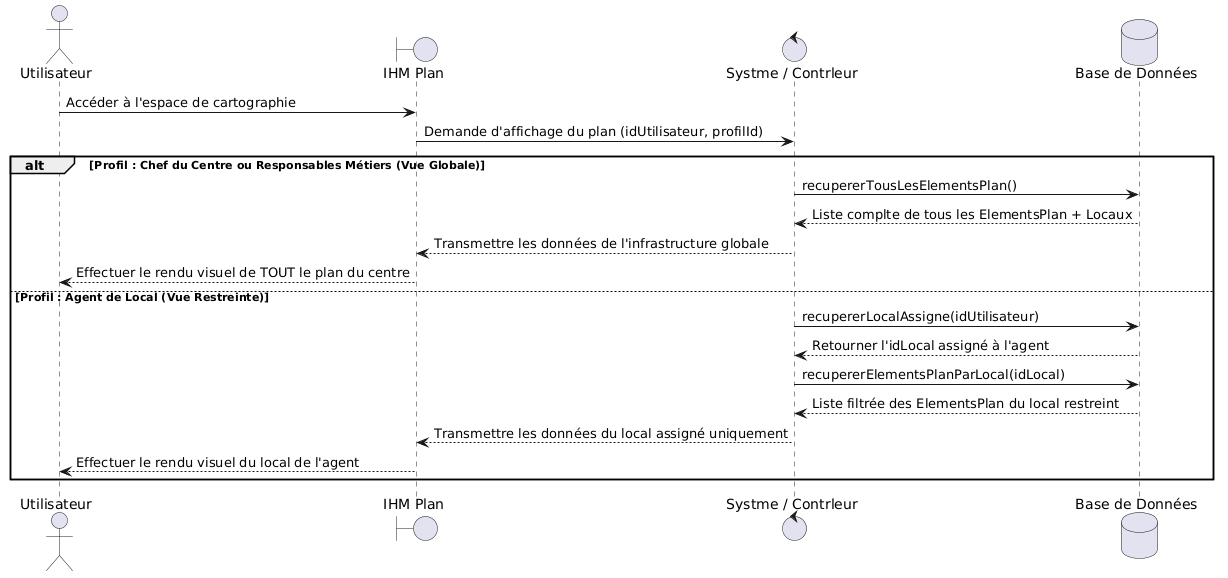
\includegraphics[width=\textwidth,height=0.65\textheight,keepaspectratio]{../../assets/seq_voir_plan.png}
  \caption{Diagramme de séquence - Visualisation du plan}
  \label{fig:seq_voir_plan}
\end{figure}

\clearpage
\subsection{Scénario de Gestion et d'Enregistrement Intermédiaire (UC\_CRUD\_Equip)}

Ce diagramme illustre la règle métier stricte du système : toute donnée brute d'équipement ou d'immobilisation créée par le responsable doit obligatoirement être enregistrée au sein de la table magasin avant de pouvoir être exploitée lors de la phase de cartographie.

\begin{figure}[H]
  \centering
  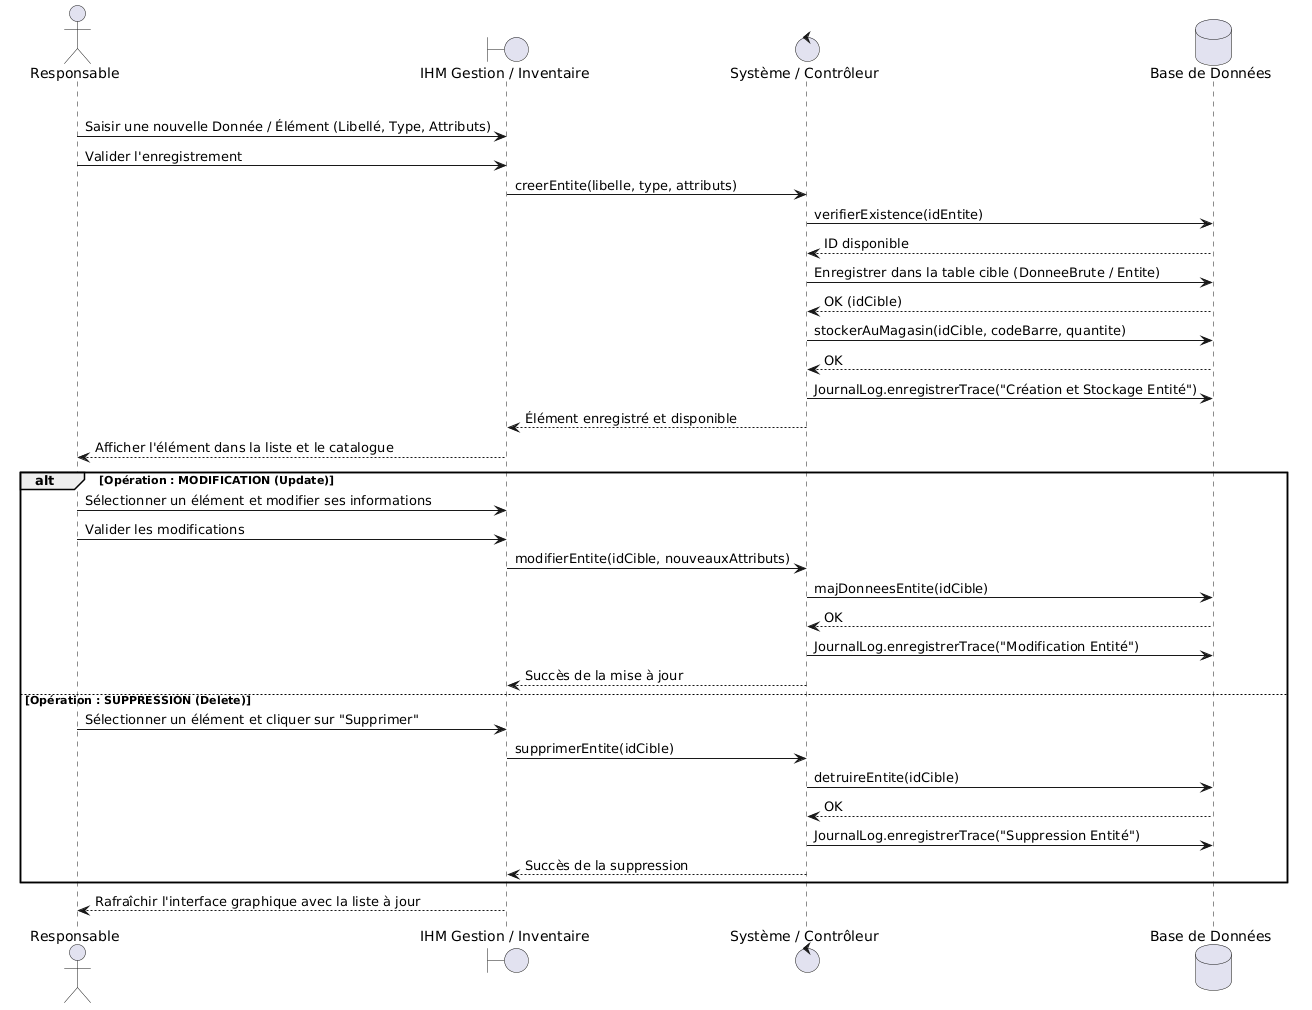
\includegraphics[width=\textwidth,height=0.65\textheight,keepaspectratio]{../../assets/seq_crud.png}
  \caption{Diagramme de séquence - Enregistrement en magasin}
  \label{fig:seq_crud_equip}
\end{figure}

\clearpage
\subsection{Scénario de Placement Spatial par Glisser-Déposer (UC\_DragDrop\_Immo)}

L'aspect dynamique du positionnement graphique traduit l'interaction de l'utilisateur avec l'interface interactive. Le contrôleur instancie un élément de plan aux coordonnées $(X, Y)$ spécifiées et met à jour la base de données en temps réel.

\begin{figure}[H]
  \centering
  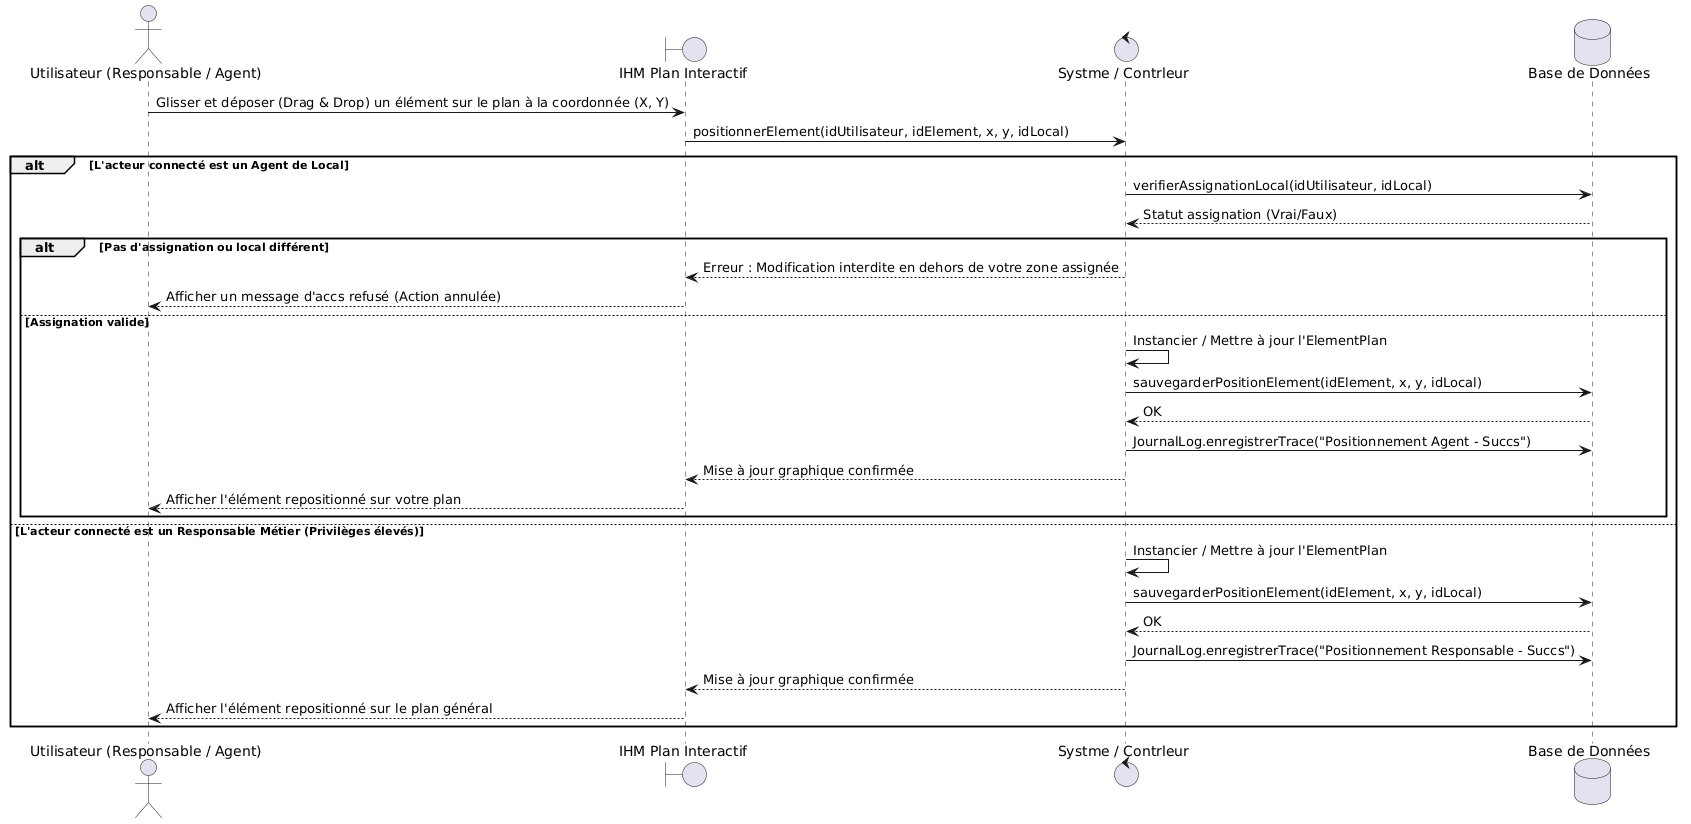
\includegraphics[width=\textwidth,height=0.65\textheight,keepaspectratio]{../../assets/seq_drag_drop.png}
  \caption{Diagramme de séquence - Placement des éléments sur le plan}
  \label{fig:seq_drag_drop}
\end{figure}

\clearpage
\subsection{Scénario de Gestion et de Notification des Pannes (UC\_Alertes)}

Le processus de déclaration d'une panne déclenche un mécanisme d'aiguillage automatique. Selon la nature de l'entité ciblée (matériel technique ou véhicule), le système identifie et notifie le responsable métier concerné tout en historisant l'incident.

\begin{figure}[H]
  \centering
  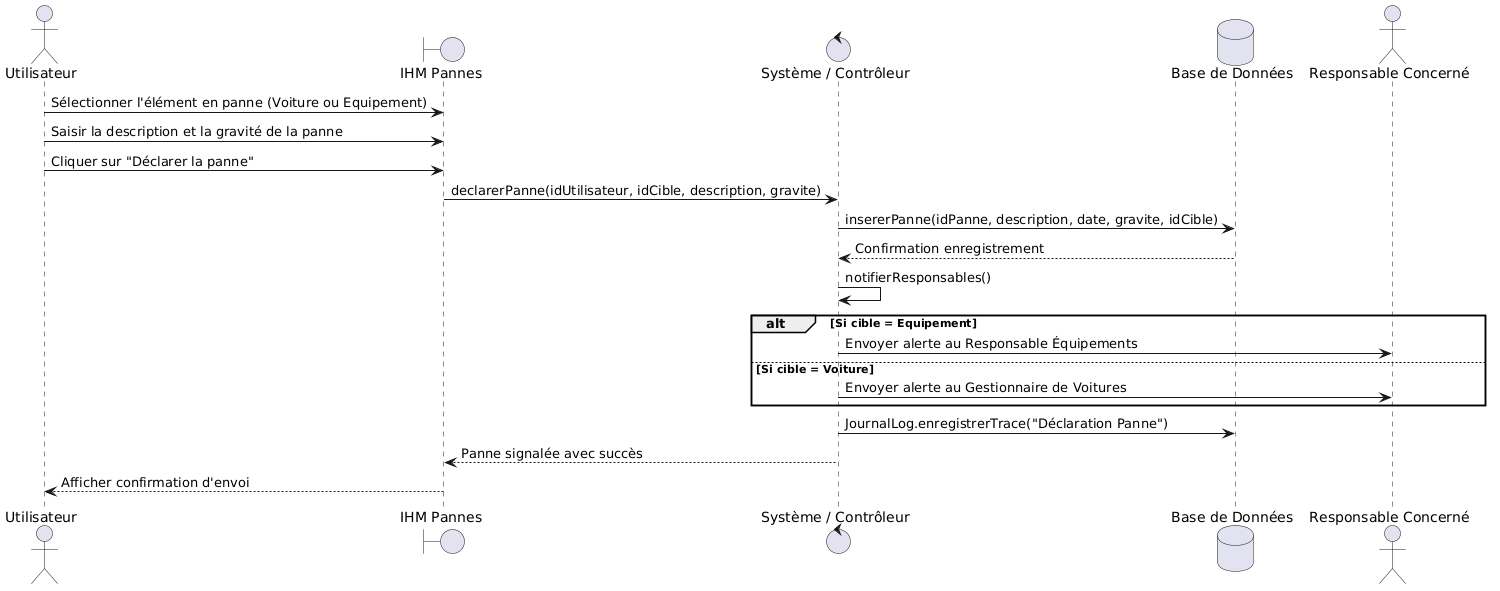
\includegraphics[width=\textwidth,height=0.65\textheight,keepaspectratio]{../../assets/seq_alertes.png}
  \caption{Diagramme de séquence - Déclaration et routage d'une alerte panne}
  \label{fig:seq_alertes}
\end{figure}

\clearpage
\subsection{Scénario de Génération Globale de Rapports (UC\_PDF)}

Conformément à l'extension des droits d'accès à l'ensemble du personnel de la STEG, ce scénario décrit la collecte transverse des données applicatives, leur compilation au format PDF et l'interrogation du journal de log à des fins d'audit de l'action.

\begin{figure}[H]
  \centering
  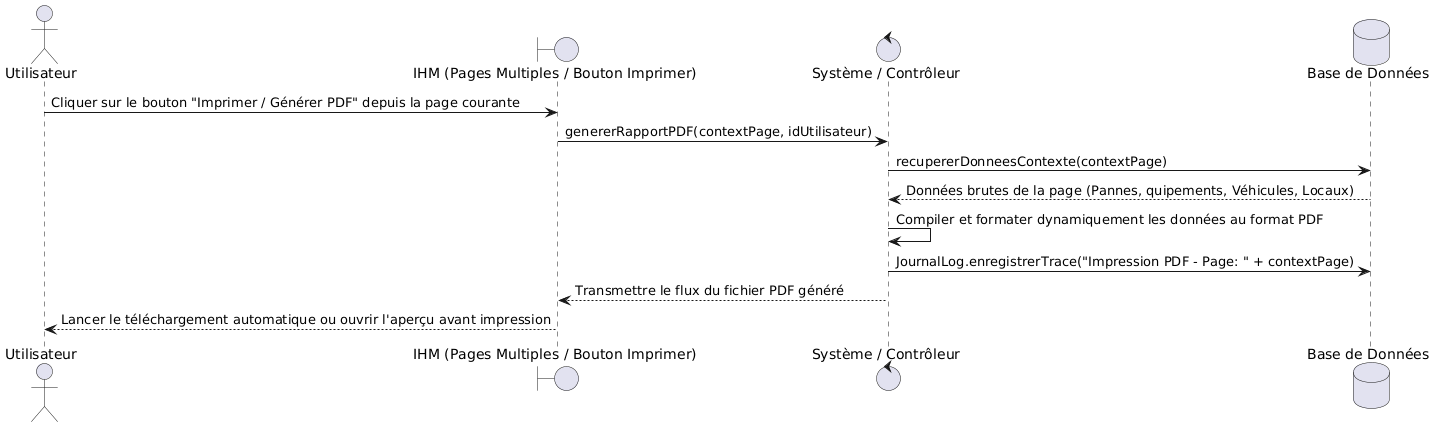
\includegraphics[width=\textwidth,height=0.65\textheight,keepaspectratio]{../../assets/seq_pdf.png}
  \caption{Diagramme de séquence - Génération de rapports PDF}
  \label{fig:seq_pdf}
\end{figure}

\clearpage
\section{Conclusion du Chapitre}

La phase de modélisation présentée dans ce chapitre a permis de figer l'ensemble des interactions et des structures nécessaires à la réalisation de l'application de gestion des immobilisations de la STEG. L'alignement rigoureux entre les cas d'utilisation, l'architecture statique des classes et la cinématique des diagrammes de séquences assure une transition fluide et sécurisée vers la phase de développement et d'implémentation technique.

\clearpage
\chapter{Réalisation et Implémentation}

\section{Introduction}

Ce chapitre est dédié à la concrétisation matérielle et logicielle du système de gestion des immobilisations. Après avoir validé les phases d'analyse et de conception, la phase de réalisation permet de traduire les modèles théoriques en composants applicatifs fonctionnels. L'étude aborde l'architecture logicielle globale retenue pour structurer le code source, détaille l'organisation de la base de données relationnelle, puis présente les principales interfaces graphiques développées afin d'illustrer la prise en main et le comportement opérationnel de l'application.

\section{Architecture Globale de l'Application}

Pour garantir la maintenabilité, la sécurité et l'évolutivité du système, le développement s'est appuyé sur une architecture modulaire et une séparation stricte des responsabilités. Le traitement des requêtes s'effectue via une logique serveur robuste en PHP qui interagit de manière sécurisée avec le système de gestion de base de données MySQL. L'interface utilisateur repose sur une intégration fluide des technologies web standards, permettant un rendu dynamique des données, une validation des formulaires côté client et une navigation fluide entre les différents modules sans rechargement lourd des pages, optimisant ainsi l'expérience d'utilisation des agents de la structure.

\section{Implémentation de la Base de Données}

La structure physique des données a été déployée sur le serveur local conformément aux spécifications du diagramme de classes. Les tables ont été optimisées avec des clés primaires et secondaires appropriées afin de garantir l'intégrité référentielle, notamment pour l'arborescence des locaux, les affectations des véhicules et le suivi du matériel électrique. L'administration et la vérification de la cohérence des enregistrements ont été assurées de manière centralisée, validant la persévérance et la sécurité des données applicatives.

\section{Présentation des Interfaces Graphiques}

L'interface graphique a été conçue pour offrir une navigation moderne, sobre et intuitive, adaptée aux besoins quotidiens des différents profils d'utilisateurs de la société.

\subsection{Interface d'Authentification}

L'accès à l'application est protégé par une page de connexion sécurisée qui constitue la porte d'entrée unique du système. Cette interface filtre les accès en vérifiant les identifiants saisis dans la table des utilisateurs afin de rediriger chaque agent vers son espace de travail personnalisé.

\begin{figure}[H]
  \centering
  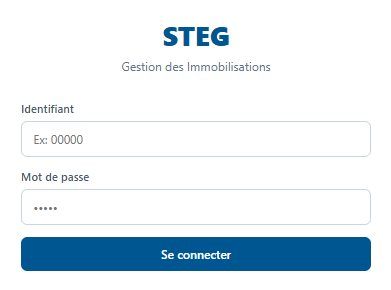
\includegraphics[width=0.9\textwidth]{../../assets/Authentification.png}
  \caption{Interface d'authentification}
  \label{fig:login_page}
\end{figure}

\subsection{Tableau de Bord Principal et Modules Associés}

Une fois l'authentification validée, le système affiche un tableau de bord centralisé qui offre une vue d'ensemble sur l'état du patrimoine. Cette page présente des indicateurs de synthèse sur le volume des immobilisations, la répartition des véhicules et les alertes d'inventaire en cours. Depuis ce tableau de bord, l'utilisateur accède aux différents modules fonctionnels de l'application.

\begin{figure}[H]
  \centering
  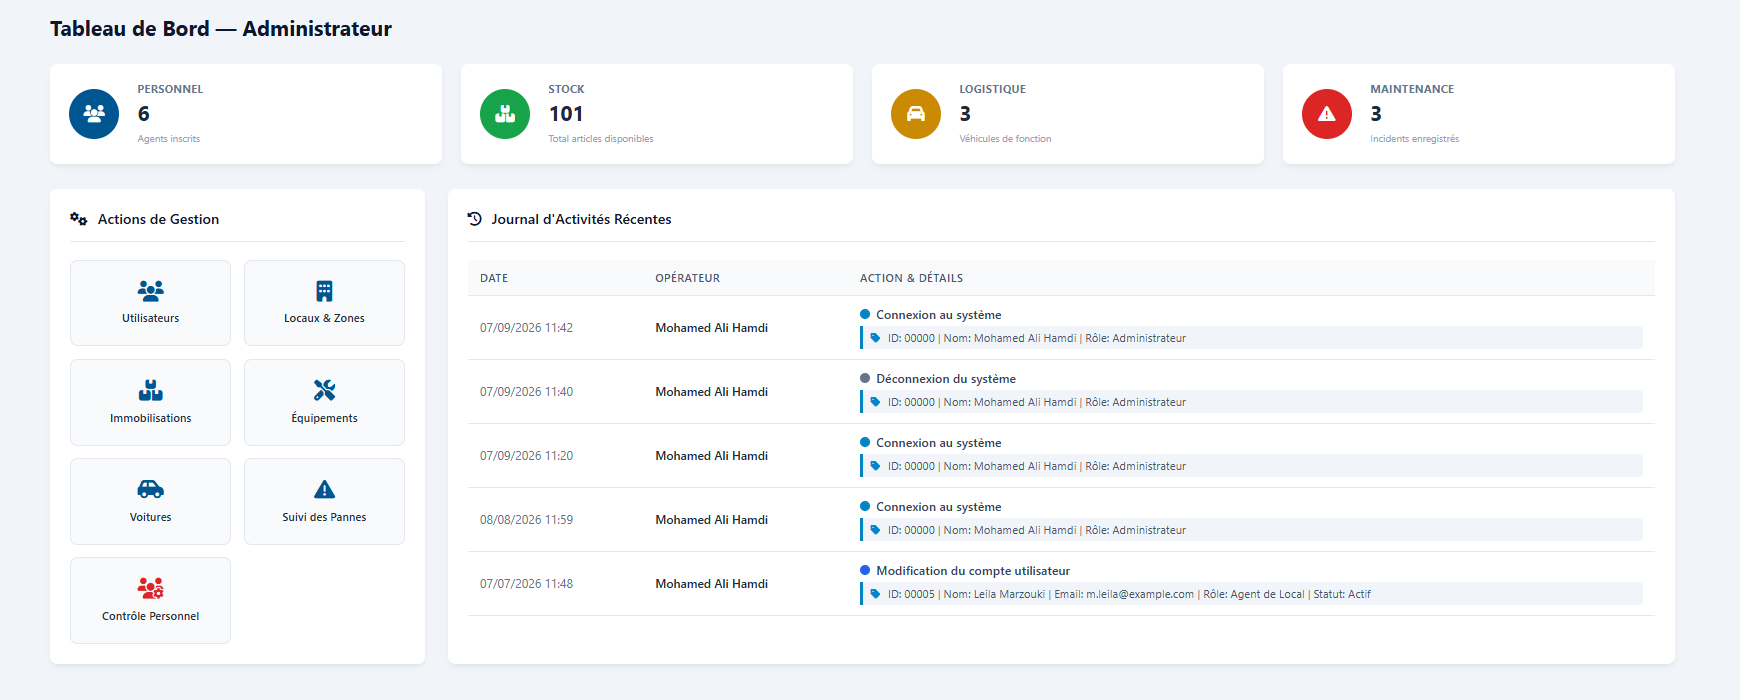
\includegraphics[width=0.9\textwidth]{../../assets/Dashboard.png}
  \caption{Tableau de bord de l'application}
  \label{fig:dashboard}
\end{figure}

\subsection{Module de Gestion des Utilisateurs}

\paragraph{Liste des Personnels}
Cette vue présente l'annuaire complet des agents enregistrés dans le système. Elle permet de visualiser rapidement les informations de contact, le département d'affectation ainsi que le rôle attribué à chaque utilisateur au sein de la plateforme.

\begin{figure}[H]
  \centering
  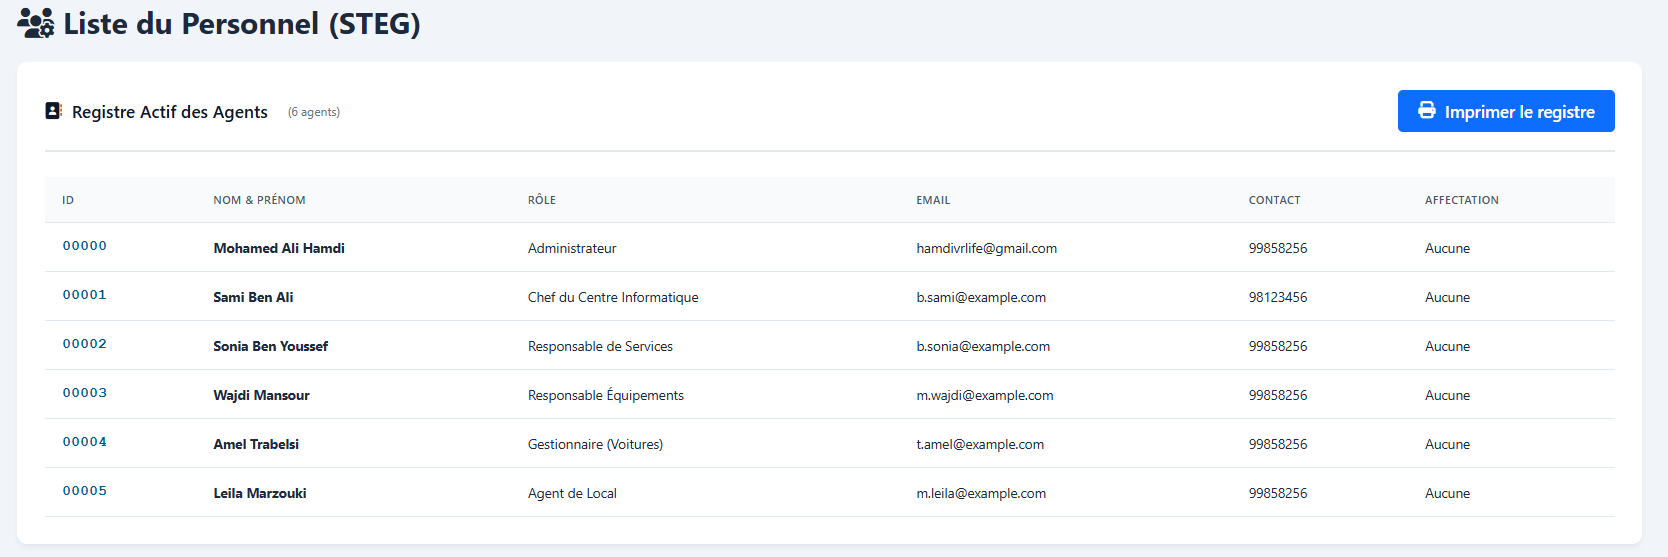
\includegraphics[width=0.9\textwidth]{../../assets/list_utilisateurs.png}
  \caption{Interface d'affichage de la liste des personnels}
  \label{fig:list_utilisateurs}
\end{figure}

\paragraph{Gestion des Personnels}
Cette interface administrative est dédiée à la création, à la modification et à la suppression des comptes utilisateurs. Elle permet également d'assigner les différents privilèges d'accès pour sécuriser les actions réalisables selon chaque profil.

\begin{figure}[H]
  \centering
  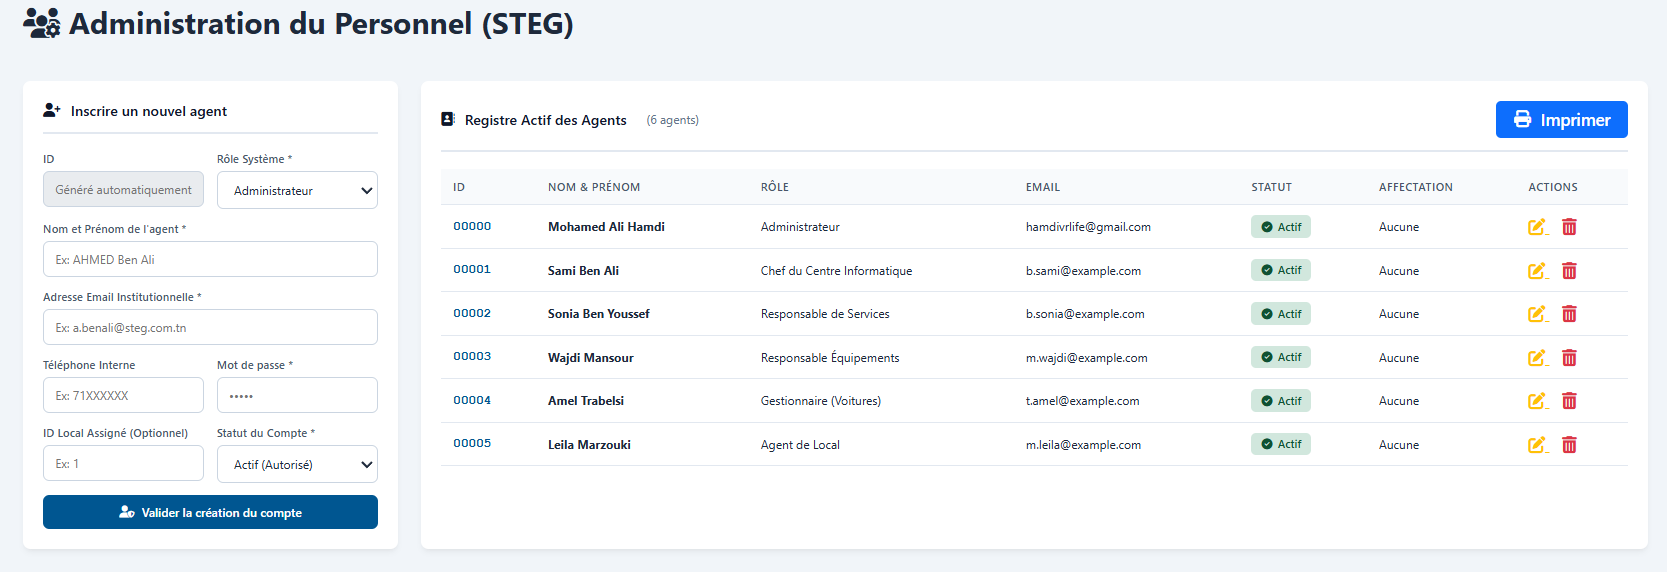
\includegraphics[width=0.9\textwidth]{../../assets/gestion_utilisateurs.png}
  \caption{Interface de gestion et d'administration des personnels}
  \label{fig:gestion_utilisateurs}
\end{figure}

\subsection{Module de Gestion des Locaux}

Ce module permet de structurer et d'administrer l'arborescence des différents bâtiments et salles de la structure. Il facilite le rattachement géographique des équipements et du personnel, garantissant ainsi une traçabilité spatiale rigoureuse de l'ensemble du patrimoine immobilier.

\begin{figure}[H]
  \centering
  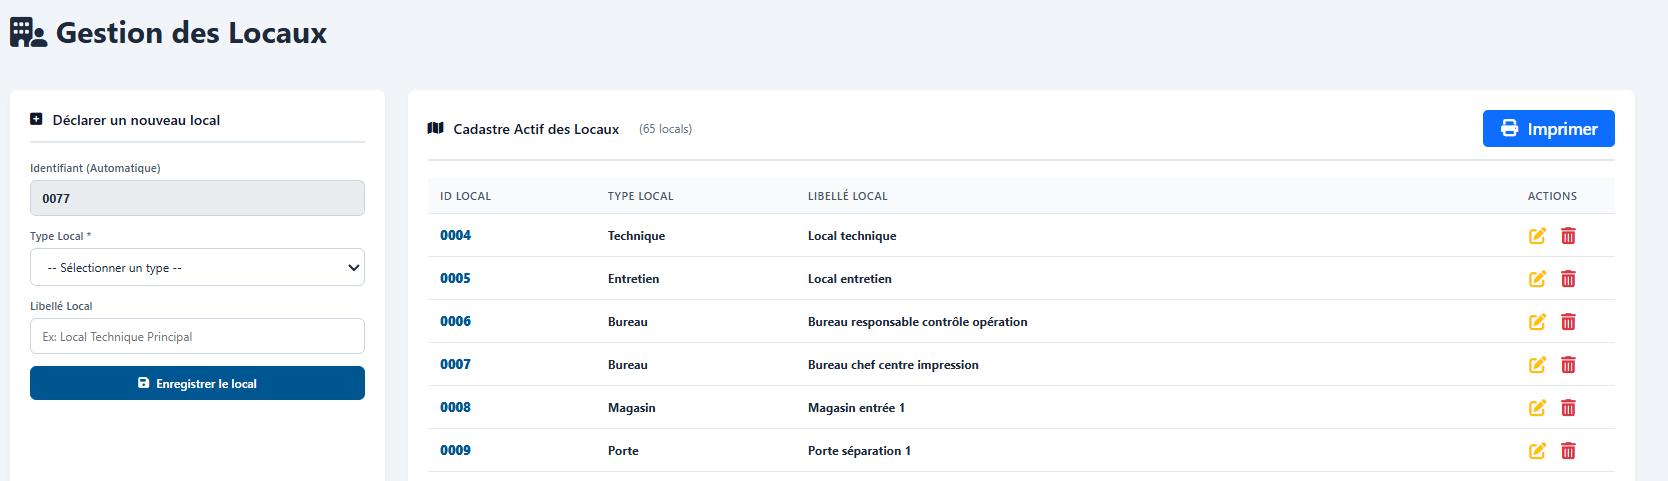
\includegraphics[width=0.9\textwidth]{../../assets/gestion_locaux.png}
  \caption{Interface de gestion des locaux}
  \label{fig:gestion_locaux}
\end{figure}

\subsection{Module de Gestion des Immobilisations}

Véritable cœur de l'application, ce module centralise l'inventaire général des biens de l'entreprise. Il permet l'enregistrement, la mise à jour et le suivi des fiches d'immobilisation, facilitant ainsi la gestion des acquisitions et la valorisation globale du patrimoine.

\begin{figure}[H]
  \centering
  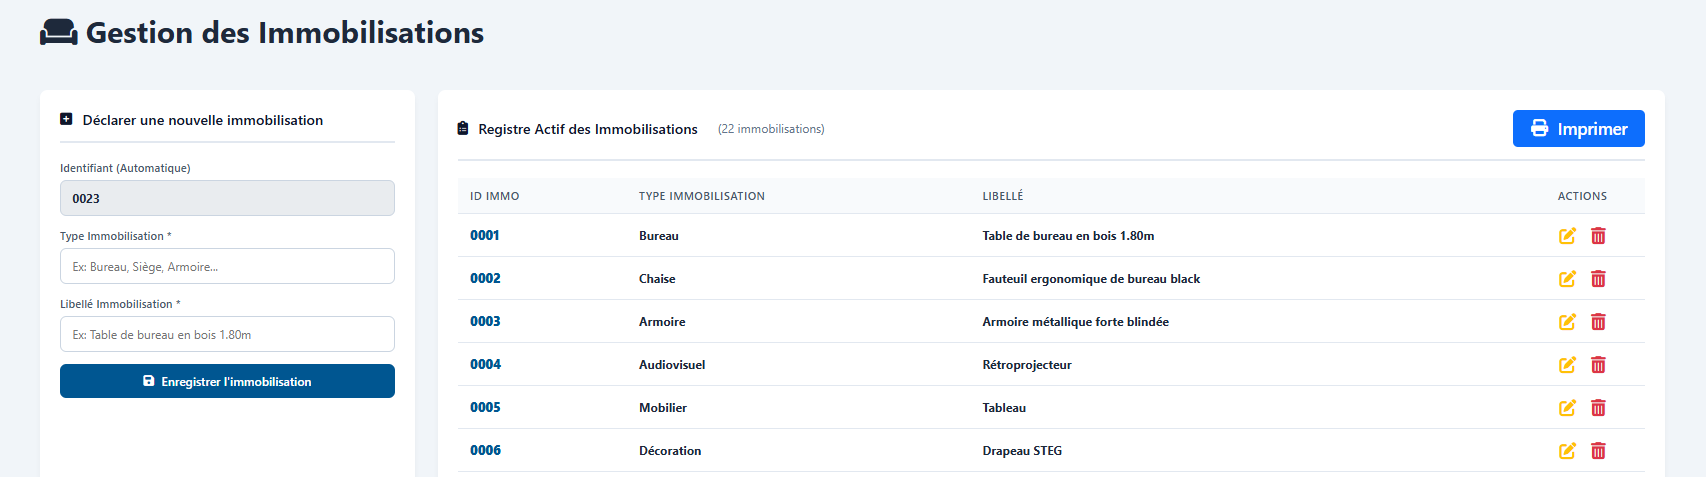
\includegraphics[width=0.9\textwidth]{../../assets/gestion_immobilisations.png}
  \caption{Interface de gestion des immobilisations}
  \label{fig:gestion_immobilisations}
\end{figure}

\subsection{Module de Suivi des Équipements}

Dédiée à la traçabilité des équipements techniques, cette vue permet d'enregistrer les équipements et de modifier leur état opérationnel, tout en conservant un historique fiable des mouvements.

\begin{figure}[H]
  \centering
  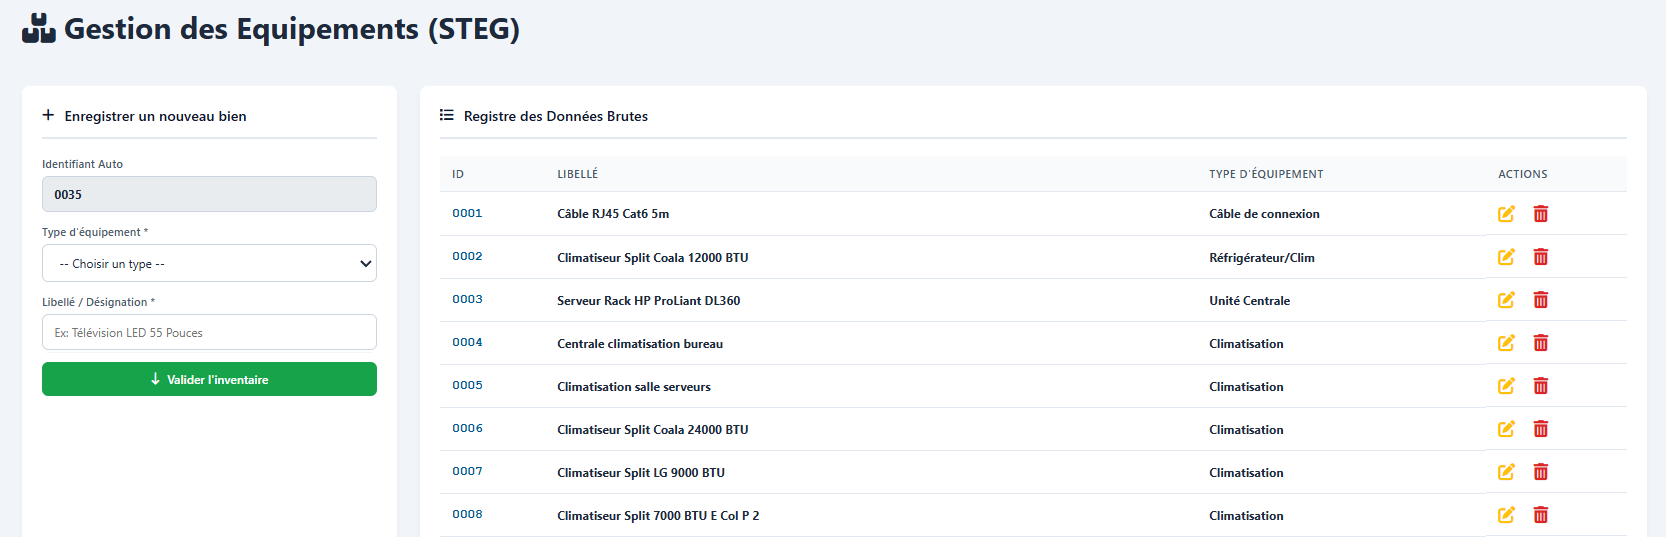
\includegraphics[width=0.9\textwidth]{../../assets/gestion_equipements.png}
  \caption{Interface de gestion des équipements}
  \label{fig:gestion_equipements}
\end{figure}

\subsection{Module de Gestion du Parc Automobile}

Cette section de l'application centralise l'ensemble des informations relatives à la flotte de véhicules de la société. Il permet le suivi des fiches techniques des voitures, de leur état général ainsi que de leurs directions d'affectation respectives.

\begin{figure}[H]
  \centering
  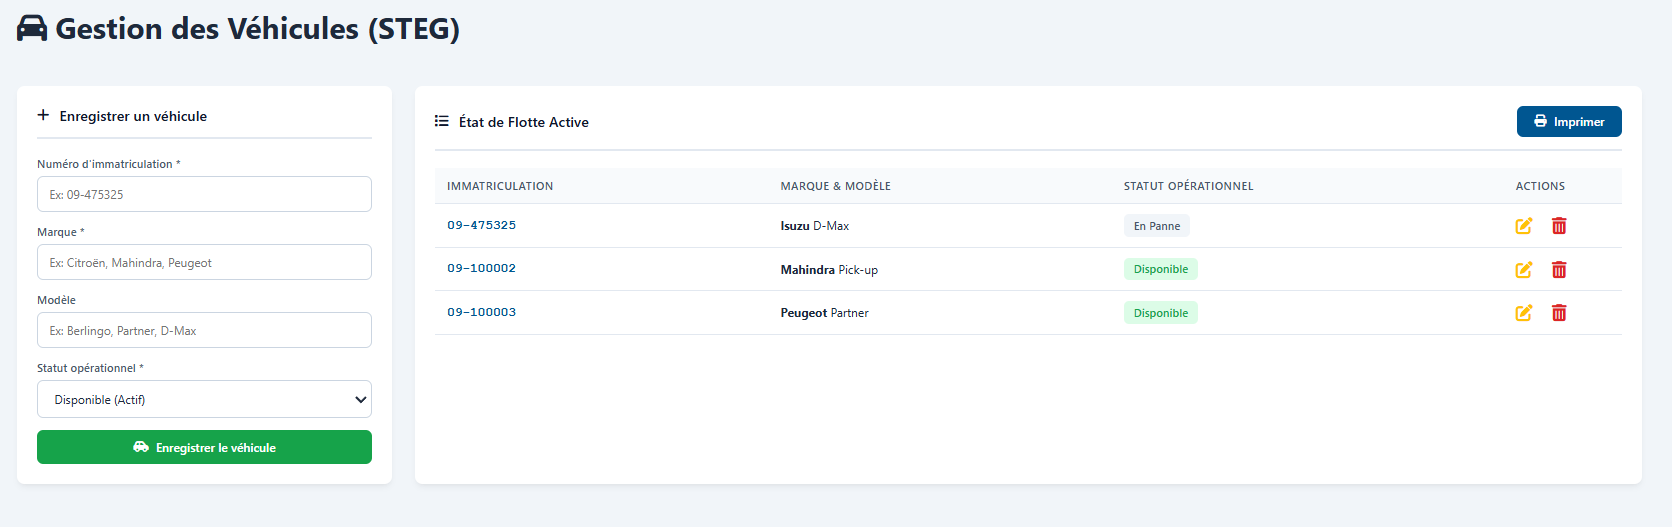
\includegraphics[width=0.9\textwidth]{../../assets/gestion_vehicules.png}
  \caption{Interface de suivi du parc roulant}
  \label{fig:gestion_vehicules}
\end{figure}

\subsection{Module de Gestion des Pannes}

Ce module est indispensable pour le suivi des dysfonctionnements signalés sur le matériel et les véhicules. Il permet de déclarer une nouvelle panne, d'attribuer un niveau de priorité, d'assurer le suivi des interventions de maintenance et de clôturer les tickets une fois la réparation effectuée.

\begin{figure}[H]
  \centering
  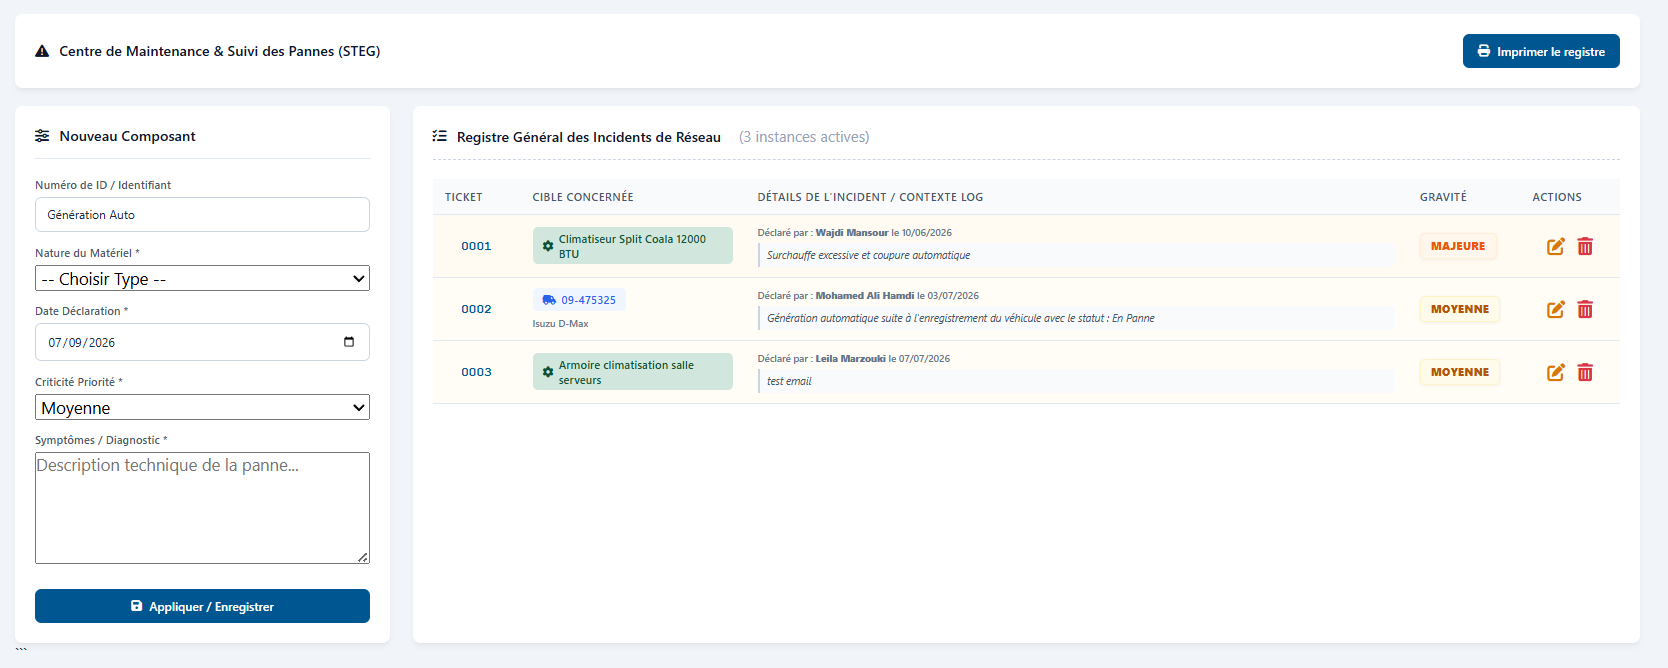
\includegraphics[width=0.9\textwidth]{../../assets/gestion_pannes.png}
  \caption{Interface de suivi des pannes}
  \label{fig:gestion_pannes}
\end{figure}

\subsection{Module de Gestion du Magasin}

Ce module gère les stocks de pièces de rechange et de matériel disponible en réserve. Il permet d'assurer un suivi rigoureux des entrées, des sorties et des seuils d'alerte des articles stockés.

\begin{figure}[H]
  \centering
  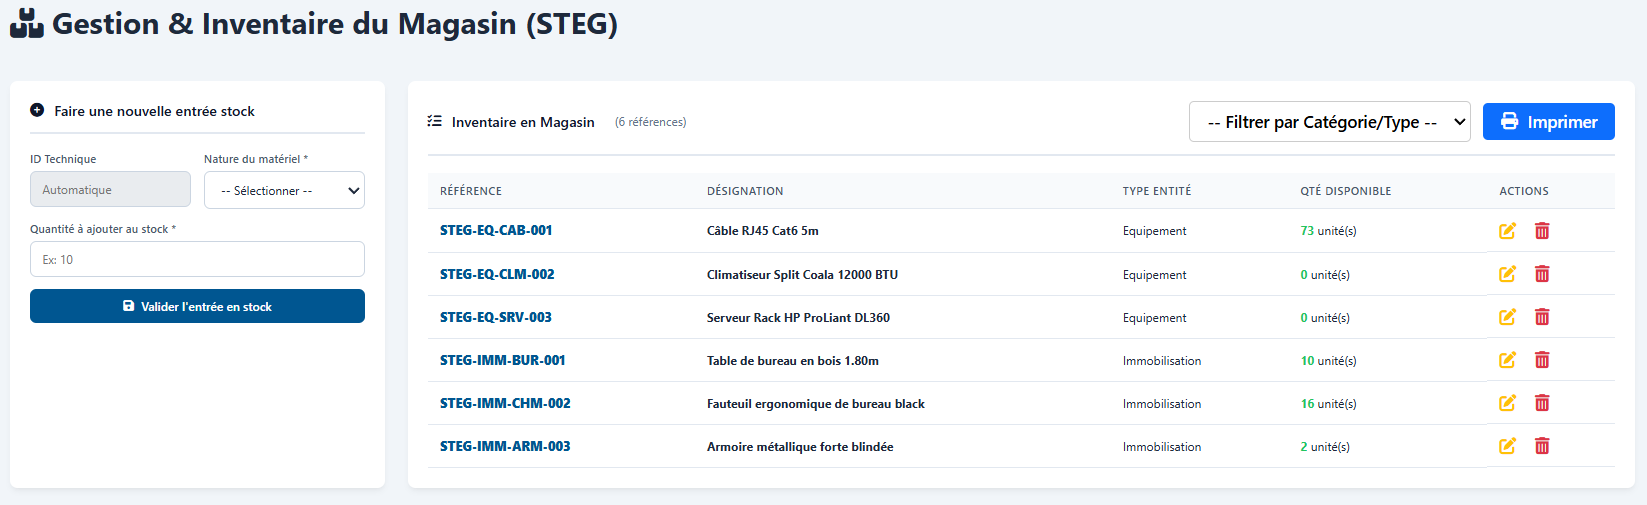
\includegraphics[width=0.9\textwidth]{../../assets/gestion_magasin.png}
  \caption{Interface de suivi du magasin}
  \label{fig:gestion_magasin}
\end{figure}

\subsection{Module de Gestion du Plan}

Cette section permet d'intégrer et de visualiser les plans architecturaux de la structure. Elle facilite la localisation interactive des immobilisations et des équipements directement sur les schémas des différents étages ou bâtiments.

\begin{figure}[H]
  \centering
  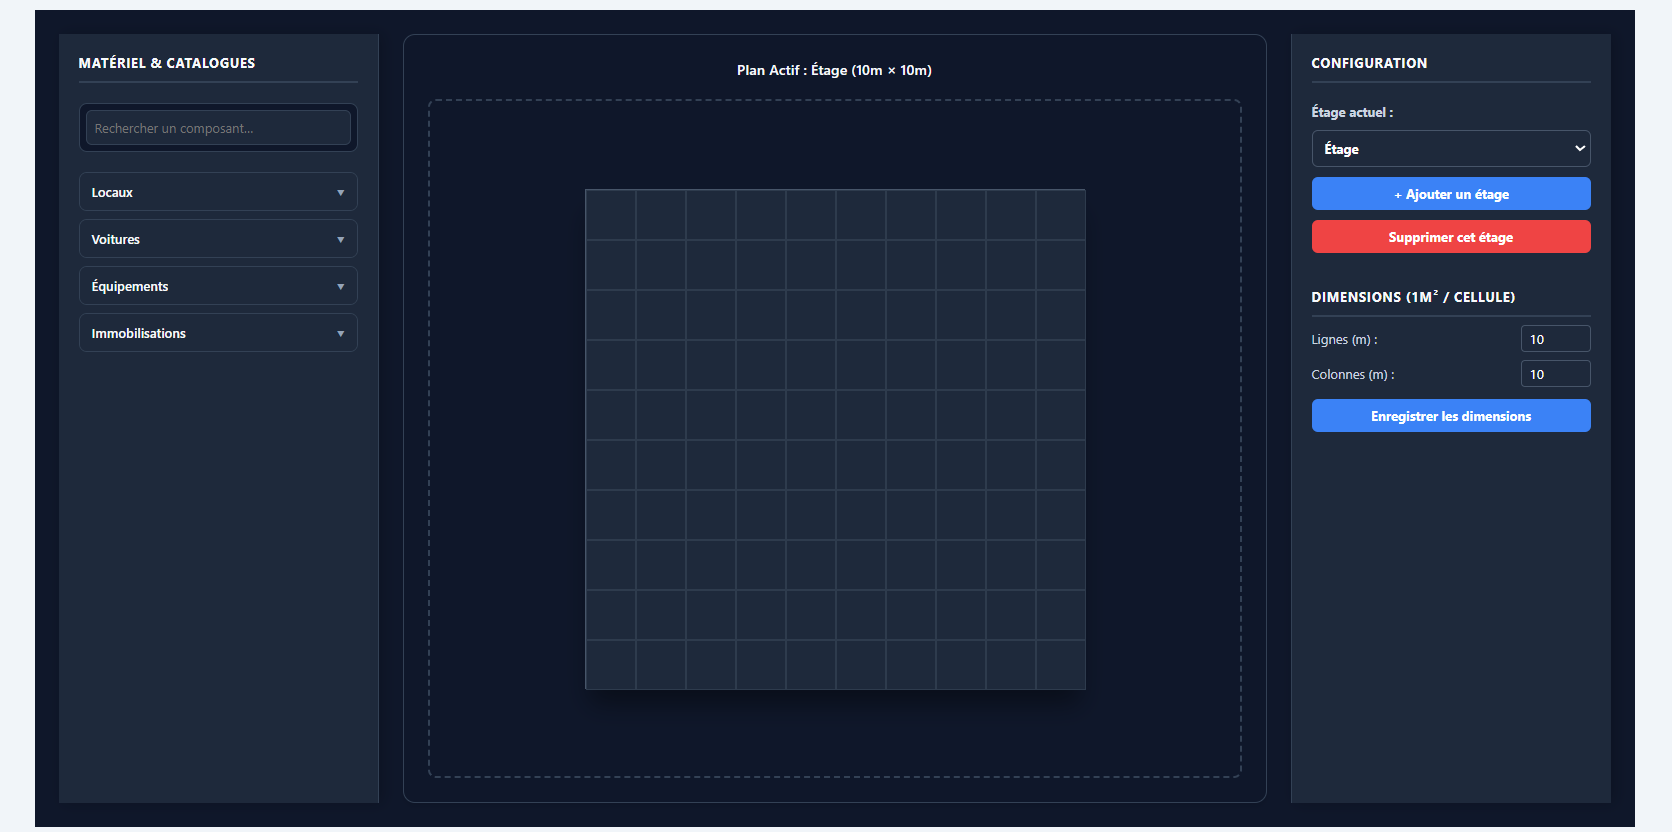
\includegraphics[width=0.9\textwidth]{../../assets/gestion_plan.png}
  \caption{Interface de suivi du plan}
  \label{fig:gestion_plan}
\end{figure}

\subsection{Module de Documentation}

Ce module centralise les guides d'utilisation, les manuels techniques et les historiques d'activité liés au système. Il permet de consulter ou de télécharger rapidement les ressources et journaux nécessaires à la bonne administration de la plateforme.

\begin{figure}[H]
  \centering
  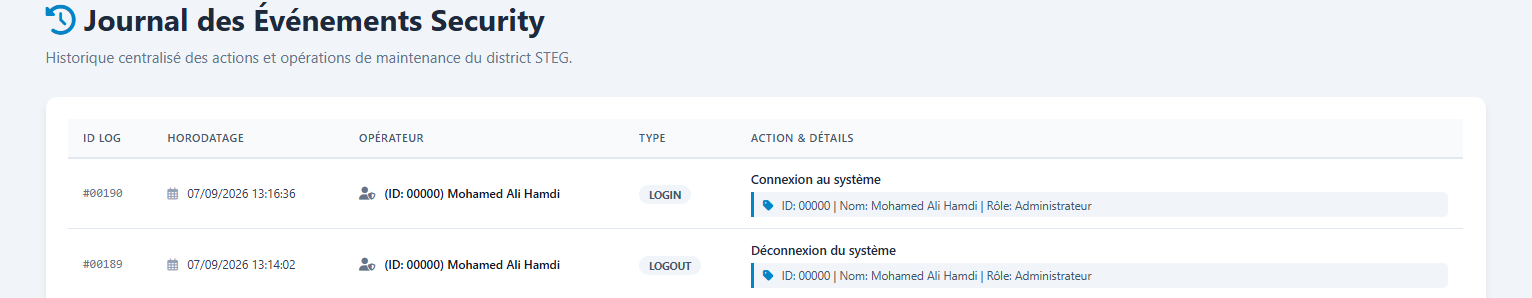
\includegraphics[width=0.9\textwidth]{../../assets/logs.png}
  \caption{Interface de gestion de la documentation}
  \label{fig:logs}
\end{figure}

\section{Conclusion du Chapitre}

En somme, cette phase de réalisation a permis de concrétiser l'ensemble des choix architecturaux et fonctionnels retenus lors de la conception. À travers le développement des différents modules, l'application offre désormais une solution opérationnelle, ergonomique et sécurisée pour la gestion globale du patrimoine. Le prochain chapitre sera consacré aux tests finaux et à la validation générale du projet.

\clearpage
\chapter*{Conclusion Générale}
\addcontentsline{toc}{chapter}{Conclusion Générale}

Le projet de fin d'année présenté tout au long de ce rapport s'est articulé autour de la conception et du développement d'une application web dédiée à la gestion des immobilisations pour la Société Tunisienne de l'Électricité et du Gaz. L'objectif initial consistait à répondre à une problématique concrète de suivi et de centralisation du patrimoine matériel, informatique et roulant, afin de pallier les limites des méthodes de gestion traditionnelles.

Les différentes étapes menées à bien ont permis d'aboutir à une solution logicielle fonctionnelle et sécurisée. La phase d'analyse des exigences a posé les bases indispensables en identifiant avec précision les besoins des différents services et profils d'utilisateurs. L'étape de conception, appuyée sur une modélisation rigoureuse des structures et des processus, a garanti l'élaboration d'une architecture de base de données relationnelle stable et cohérente. Enfin, la phase d'implémentation a concrétisé ces travaux à travers une interface web intuitive, interconnectée à une logique applicative robuste capable d'assurer la traçabilité complète de chaque actif au sein des locaux.

Sur le plan personnel et technique, ce travail a constitué une opportunité d'approfondir et de consolider des compétences pratiques en développement complet et en gestion de bases de données, tout en se confrontant aux réalités opérationnelles et aux exigences de sécurité d'une grande entreprise publique nationale. L'immersion au sein du Département d'Exploitation Informatique Sud a permis de comprendre l'importance d'une planification structurée et d'une conception modulaire pour garantir la réussite d'un projet informatique.

Bien que l'application réponde aux spécifications établies dans le cahier des charges, le système reste ouvert à de futures extensions opérationnelles. En guise de perspectives, l'intégration d'un module de notification automatique pourrait être envisagée pour planifier les opérations de maintenance préventive du matériel électrique et le contrôle technique des véhicules. De plus, l'adoption de technologies d'identification rapide, telles que la génération et la lecture de codes-barres ou de codes QR pour chaque immobilisation, permettrait d'automatiser entièrement le processus de contrôle physique lors des campagnes d'inventaire annuel.

\end{document}